\documentclass[12pt,]{book}
\usepackage{lmodern}
\usepackage{amssymb,amsmath}
\usepackage{ifxetex,ifluatex}
\usepackage{fixltx2e} % provides \textsubscript
\ifnum 0\ifxetex 1\fi\ifluatex 1\fi=0 % if pdftex
  \usepackage[T1]{fontenc}
  \usepackage[utf8]{inputenc}
\else % if luatex or xelatex
  \ifxetex
    \usepackage{mathspec}
  \else
    \usepackage{fontspec}
  \fi
  \defaultfontfeatures{Ligatures=TeX,Scale=MatchLowercase}
\fi
% use upquote if available, for straight quotes in verbatim environments
\IfFileExists{upquote.sty}{\usepackage{upquote}}{}
% use microtype if available
\IfFileExists{microtype.sty}{%
\usepackage{microtype}
\UseMicrotypeSet[protrusion]{basicmath} % disable protrusion for tt fonts
}{}
\usepackage[margin=1in]{geometry}
\usepackage{hyperref}
\hypersetup{unicode=true,
            pdftitle={Challenges and Tools in the Assessment and Management of Pacific Salmon Fisheries},
            pdfauthor={Ben Staton},
            pdfborder={0 0 0},
            breaklinks=true}
\urlstyle{same}  % don't use monospace font for urls
\usepackage{natbib}
\bibliographystyle{apalike}
\usepackage{longtable,booktabs}
\usepackage{graphicx,grffile}
\makeatletter
\def\maxwidth{\ifdim\Gin@nat@width>\linewidth\linewidth\else\Gin@nat@width\fi}
\def\maxheight{\ifdim\Gin@nat@height>\textheight\textheight\else\Gin@nat@height\fi}
\makeatother
% Scale images if necessary, so that they will not overflow the page
% margins by default, and it is still possible to overwrite the defaults
% using explicit options in \includegraphics[width, height, ...]{}
\setkeys{Gin}{width=\maxwidth,height=\maxheight,keepaspectratio}
\IfFileExists{parskip.sty}{%
\usepackage{parskip}
}{% else
\setlength{\parindent}{0pt}
\setlength{\parskip}{6pt plus 2pt minus 1pt}
}
\setlength{\emergencystretch}{3em}  % prevent overfull lines
\providecommand{\tightlist}{%
  \setlength{\itemsep}{0pt}\setlength{\parskip}{0pt}}
\setcounter{secnumdepth}{5}
% Redefines (sub)paragraphs to behave more like sections
\ifx\paragraph\undefined\else
\let\oldparagraph\paragraph
\renewcommand{\paragraph}[1]{\oldparagraph{#1}\mbox{}}
\fi
\ifx\subparagraph\undefined\else
\let\oldsubparagraph\subparagraph
\renewcommand{\subparagraph}[1]{\oldsubparagraph{#1}\mbox{}}
\fi

%%% Use protect on footnotes to avoid problems with footnotes in titles
\let\rmarkdownfootnote\footnote%
\def\footnote{\protect\rmarkdownfootnote}

%%% Change title format to be more compact
\usepackage{titling}

% Create subtitle command for use in maketitle
\newcommand{\subtitle}[1]{
  \posttitle{
    \begin{center}\large#1\end{center}
    }
}

\setlength{\droptitle}{-2em}

  \title{Challenges and Tools in the Assessment and Management of Pacific Salmon
Fisheries}
    \pretitle{\vspace{\droptitle}\centering\huge}
  \posttitle{\par}
    \author{Ben Staton}
    \preauthor{\centering\large\emph}
  \postauthor{\par}
    \date{}
    \predate{}\postdate{}
  
\usepackage{booktabs}
%%% This is an example file for the Auburn University style options
%%%       aums.sty (Masters Thesis)
%%%       auphd.sty (Ph.D. Dissertation)
%%%       auhonors.sty (Honors Scholar)

%%%To use it, please edit the necessary options, title, author, date, year, keywords, advisor, professor, etc. 

% \documentclass[12pt]{report}
\usepackage{setspace}
% \usepackage{titlesec}
%\setcounter{secnumdepth}{3}
% \usepackage{aums}       % For Master's papers
\usepackage{auphd}     % For Ph.D.
%\usepackage{auhonors}  % For honors college
\usepackage[normalem]{ulem}       % underlining on style-page; see \normalem below
\usepackage{url}
\usepackage[table]{xcolor}
\usepackage{tikz}
\usepackage{pgf}

\usepackage{amsmath,amsthm, amsfonts, mathrsfs, graphicx, setspace, fullpage, color}
\usepackage{natbib, appendix}
\usepackage[T1]{fontenc}
\usepackage{multirow}
\usepackage{mathabx}
\RequirePackage{adjustbox}
% \usepackage{epstopdf}
\AtBeginDocument{\renewcommand{\bibname}{References}}
\usepackage{hyperref}
%\usepackage{tocloft}
%\renewcommand\cftchapafterpnum{\vskip\baselineskip}
%\renewcommand\cftsecafterpnum{\vskip\baselineskip}
%\renewcommand\cftsubsecafterpnum{\vskip\baselineskip}
%\renewcommand\cftsubsubsecafterpnum{\vskip\baselineskip}
%\renewcommand\cftfigafterpnum{\vskip\baselineskip}
%\renewcommand\cfttabafterpnum{\vskip\baselineskip}

%%%%%Format rules: Normal margins are 1 in. If you need to print with 1.5in margins, uncomment the line below
%\oddsidemargin0.5in \textwidth6in

%% If you do not need a List of Abbreviations, then comment out the lines below and the \printnomenclature line.
%%for List of Abbreviations information:  (see http://www.mackichan.com/TECHTALK/509.htm  )
% \usepackage[intoc]{nomencl}
% \renewcommand{\nomname}{List of Abbreviations}   	       
% \makenomenclature 
%% don't forget to run:   makeindex ausample.nlo -s nomencl.ist -o ausample.nls
%% Also, if 

\makeatother
\let\oldmaketitle\maketitle
\AtBeginDocument{\let\maketitle\relax}

% Put the title, author, and date in. 
\title{Challenges and Tools in the Assessment and Management of Pacific Salmon Fisheries}
\author{Benjamin A. Staton} 
\date{May 5, 2019} %date of graduation
\copyrightyear{2019} %copyright year

\keywords{Fisheries management, Bayesian inference, decision analysis}

% Put the Thesis Adviser here. 
\adviser{Matthew J. Catalano}

% Put the committee here (including the adviser), one \professor for each. 
% The advisor must be first, and the dean of the graduate school must be last.
\professor{Matthew J. Catalano, AFFILIATION}

\professor{Asheber Abebe, AFFILIATION}

\professor{Lewis G. Coggins, Jr., AFFILIATION}

\professor{Conor P. McGowan, AFFILIATION}
\usepackage{booktabs}
\usepackage{longtable}
\usepackage{array}
\usepackage{multirow}
\usepackage[table]{xcolor}
\usepackage{wrapfig}
\usepackage{float}
\usepackage{colortbl}
\usepackage{pdflscape}
\usepackage{tabu}
\usepackage{threeparttable}
\usepackage{threeparttablex}
\usepackage[normalem]{ulem}
\usepackage{makecell}

\usepackage{amsthm}
\newtheorem{theorem}{Theorem}[chapter]
\newtheorem{lemma}{Lemma}[chapter]
\theoremstyle{definition}
\newtheorem{definition}{Definition}[chapter]
\newtheorem{corollary}{Corollary}[chapter]
\newtheorem{proposition}{Proposition}[chapter]
\theoremstyle{definition}
\newtheorem{example}{Example}[chapter]
\theoremstyle{definition}
\newtheorem{exercise}{Exercise}[chapter]
\theoremstyle{remark}
\newtheorem*{remark}{Remark}
\newtheorem*{solution}{Solution}
\begin{document}
\maketitle

\begin{romanpages}      % roman-numbered pages 

\TitlePage 

\doublespacing
\setlength{\parskip}{0pt plus 0pt minus 0pt}

\begin{abstract} 
\noindent
I'm going to write an abstract to go here. This is the first paragraph of the dissertation abstract, which will talk about chapter 1..

This is the second paragraph of the dissertation abstract, which will talk broadly about chapter 2.

This is the third paragraph of the dissertation abstract, which will talk broadly about chapter 3.

This is the fourth paragraph of the dissertation abstract, which will talk broadly about chapter 4.
\end{abstract}

\begin{acknowledgments}
\noindent
Here is where I will thank everyone.

Matt, Lew, Brendan, Mike, Sam, AL-HPC folks, Steve, Nick, Zach, Janessa. Family and Michelle. Folks at the lab. RStudio staff.
\end{acknowledgments}

\begin{singlespace}
	\tableofcontents
	\clearpage
	\listoffigures
	\clearpage
	\listoftables
\end{singlespace}

% \printnomenclature[0.5in] %used for the List of Abbreviations
\end{romanpages}        % All done with roman-numbered pages

\normalem       % Make italics the default for \em

% \titlespacing\section{0pt}{12pt plus 4pt minus 2pt}{0pt plus 2pt minus 2pt}
% \titlespacing\subsection{0pt}{12pt plus 4pt minus 2pt}{0pt plus 2pt minus 2pt}
% \titlespacing\subsubsection{0pt}{12pt plus 4pt minus 2pt}{0pt plus 2pt minus 2pt}

\setlength{\parskip}{0pt plus 0pt minus 0pt}

\doublespacing

\chapter*{Preface}\label{preface}
\addcontentsline{toc}{chapter}{Preface}

I used bookdown \citep{xie-2015} to make this document.

\chapter{Introduction}\label{ch1}

\noindent
Pacific salmon (\emph{Oncorhynchus} spp.) constitute an integral natural
resource in Alaska to subsistence, commercial, and recreational
interests. There is a long history of resource development,
exploitation, regulation, and dependence on these resources within the
region \citep{cooley-1963}. In many cases, the resource use is dictated
by the locality of the system; for example, stocks located near urban
areas are often primarily exploited by recreational fishers whereas more
remote stocks often constitute commercial and/or subsistence uses. This
proposed dissertation focuses on the challenges and solutions in the
assessment and management of these more remote stocks and the
subsistence fisheries that rely heavily upon them.

Wild Pacific salmon represent a fantastic natural resource, which
results largely from their unique life history strategy. Pacific salmon
exhibit a migratory strategy known as anadromy: they spawn in freshwater
where eggs hatch and juveniles rear for several years. Juveniles then
migrate to the ocean where they spend the majority of their lives
feeding on abundant prey resources. Once reaching maturity, adults
return to their natal streams to spawn and complete the life cycle. The
result of this life history strategy is an incredibly productive
resource that grows entirely on its own and delivers itself to
harvesters when the time comes for exploitation.

Like for all exploited natural resources, the management of Pacific
salmon fisheries involves making decisions about how to exploit the
resource in order to best attain a suite of biological, social, and
economic objectives \citep{walters-1986}. These decisions are
intrinsically difficult due to conflicting objectives and uncertainties
in system state, system response to management actions, and
implementation \citep{walters-holling-1990}. Put another way, assuming a
manager knows exactly what they wish to obtain, getting there is made
difficult by not knowing how large the harvestable surplus is, how the
stock will respond to harvesting, or that their management action will
actually obtain what is desired. Despite these difficulties, a decision
must be made \citep[without decision-making there is no
management;][]{hilborn-walters-1992} and the consequences, whether
favorable or undesirable, must be accepted. Thus, I would argue that the
science of monitoring, assessment, and prediction in the context of
Pacific salmon fisheries is tasked with identifying trade-offs and
reducing uncertainty, both of which insert difficulty into the
decision-making process as discussed below.

The management of Pacific salmon fisheries can be thought of as a
hierarchy of (1) guiding objectives, (2) management strategies to attain
objectives, and (3) tactics to implement the management strategies
(Table \ref{tab:mgmt-hierarchy-table}). At the upper level, long-term
decisions are made about the objectives of the resource exploitation.
These long-term objectives constitute what could be referred to as
fundamental objectives: they are desired endpoints, but do not at all
imply how they should be attained. These fundamental objectives often
involve notions of sustainability and maintenance of biological
diversity and often include social objectives such as maximization and
stability of harvest. Already, it is clear that these fundamental
objectives are often conflicting. For example, consider the objective of
maximizing harvest: in fisheries that harvest multiple stocks (i.e.,
distinct spawning units), oftentimes maximum harvest may only obtained
by overexploiting weak stock components and possibly reducing diversity.
As another example, consider the objective of long-term sustainability:
in order to ensure that the stock is sustained, some level of harvest
fluctuations must be accepted (lower harvests must be allowed when the
stock is at low abundance). These conflicting objectives imply that
trade-offs exist (all objectives cannot be maximized simultaneously). It
is worth noting here that the decisions made at the uppermost level of
the management hierarchy are purely social and economic and salmon stock
assessment scientists should play little-to-no advisory or advocacy
roles in making these decisions \citep{walters-martell-2004}. The Policy
for the Management of Sustainable Salmon Fisheries (5 AAC 39.222) states
that the objectives of salmon management in Alaska are

\begin{quote}
``\ldots{}to ensure conservation of salmon and salmon's required marine
and aquatic habitats, protection of customary and traditional
subsistence uses and other uses, and the sustained economic health of
Alaska's fishing communities''.
\end{quote}

\noindent
The policy goes on to say that managers should target ``\ldots{} to the
extent possible, maximum sustained yield {[}MSY{]}''.

The second level of the management hierarchy is made up of harvest
strategies and policies that guide how the long term objectives are to
be obtained. The State of Alaska has selected the fixed escapement
policy as the management strategy to obtain the long-term objectives of
sustainability and yields that are close to the maximum. These
escapement goals are given as ranges that dictate the target number of
spawning adults each year; any portion of the stock above the escapement
goal is considered surplus (excess biological production) and should be
harvested. Uncertainty at this intermediate level of the management
hierarchy (i.e., regarding the optimal escapement goal) is often a
result of incomplete understanding of system status and function. For
example, in order to determine what the optimal escapement goal should
be to obtain MSY, knowledge of stock productivity and carrying capacity
are required. These quantities are often derived using spawner-recruit
analyses, which are inherently uncertain: data are rarely informative
about the shape of the true underlying spawner-recruit relationship but
instead provide a probabilistic distribution of expected outcomes at a
given stock size \citep{walters-martell-2004}. Traditionally, it has
been thought that these uncertainties can be reduced by more monitoring
and the development of rigorous assessment and prediction models to
better understand system function. However, it has often been argued
that while monitoring and assessment models are obviously important
(performance relative to objectives must be measured), true
understanding of system behavior comes only from experimentation in
management \citep[the concept of ``active adaptive
management'';][]{walters-1986}. The classic example is to assess the
maximum productivity of the stock (i.e., in the absence of density
dependent mortality), the spawning stock must be forced to small sizes
and the resulting recruitments must be observed. However, management
actions that ensure these observations are made are undesirable to many
managers and stakeholders, considering that exploiting a stock down to
these low levels is risky \citep{walters-1986}.

At the lower level in the management hierarchy, intra-annual (or
in-season) decisions are made regarding how to exploit the current
year's run to attain the long-term objectives. In other words, given a
management strategy (i.e., fixed escapement), the manager is still
tasked with deciding how to best implement the fishery within a year to
ensure the strategy is followed. As will be illustrated in this proposed
dissertation, these decisions at the intra-annual level of the
management hierarchy are often poorly informed by data which often
results in indecisiveness, subjectivity, non-transparency, frustration,
and missed opportunities.

This proposed dissertation will be partitioned into three chapters, each
that expands on and investigates the performance of potential solutions
to the aforementioned difficulties in Pacific management in Western
Alaska. Each chapter will focus on the Kuskokwim River drainage in
Western Alaska, which is characterized by being a large drainage
(\textgreater{}50,000 km\textsuperscript{2}), harvests are taken by
primarily subsistence users who are nearly all native Alaskans, and the
primary species of interest being Chinook salmon. Although this proposed
dissertation is quite narrow in its geographical and biological focus, a
wide range of management issues will be addressed and the developed
tools and assessment methods will be evaluated thoroughly. Furthermore,
the concepts and tools discussed, developed, and evaluated will be
generalizable to other stocks with similar spatial structures,
exploitation characteristics, and population dynamics.

Chapter \ref{ch2} will work at the intra-annual level of the hierarchy
to develop and evaluate the performance of a run timing forecast model
that can be used to aid in the interpretation of in-season data. As will
be shown, uncertainty in run timing makes the interpretation of
in-season data incredibly difficult. For example, consider a case in
which an abundance index has produced high counts early in the season
when compared to the historical average. This observation is consistent
with at least two run scenarios: (1) a small run with early run timing
or (2) a large run with average timing. There is a large discrepancy in
the amount of harvestable surplus suggested by each of these discrete
scenarios, leading to a large amount of uncertainty about how the
fishery should be executed. The overall objective of Chapter \ref{ch2}
will be to develop and evaluate the reliability of a run timing forecast
model for Kuskokwim River Chinook salmon. A secondary goal of Chapter
\ref{ch2} will be to formally assess the utility of having access to the
run timing forecast model in terms of reducing uncertainty and bias in
run size indices used in intra-annual management decisions.

Chapter \ref{ch3} will again address the lowest level of the management
hierarchy (i.e., intra-annual decision-making), but in this case in a
more direct sense using an analysis framework known broadly as
Management Strategy Evaluation (MSE). This analysis will seek to
evaluate several harvest control tactics to identify strategies that
perform well at attaining pre-defined objectives (e.g., meeting the
escapement goal, distributing harvest equally across villages and stock
components, etc.) across a range of biological states (e.g., run size,
stock composition, and run timing). This analysis is needed because
while the fixed escapement strategy seems simple to execute, actually
doing so is made difficult largely due to uncertainty regarding the size
of the incoming run (i.e., the amount of harvestable surplus is not
known). Additionally, there may be a set of tactics that perform well at
limiting harvest in low run size years but doing so in a ``fair way',
where the burdens of shortages aren't carried primarily by a certain
subset of resource users. If a consistent set of rules or triggers could
be identified that perform reasonably well at meeting management
objectives without precise knowledge of run size, it could prove very
useful to managers and decision making within the region.

Chapter \ref{ch4} will move up the hierarchy to the second level and
will seek to extend the single stock assessment models currently used in
many systems in Alaska to multi-stock assessments. When an aggregate
stock is made up of several distinct components, each with their own
productivity, it is likely that exploitation at some level (e.g., 50\%)
results in the more productive components being under-exploited while
the weaker stocks may be over-exploited. This reality implies a
trade-off: to preserve stock diversity, some harvest must be foregone.
Before the shape and magnitude of these types of
``harvest-biodiversity'' trade-offs are quantified, some understanding
of the variation in substock productivity and carrying capacity is
required. The multi-stock assessment framework developed in Chapter
\ref{ch4} will be tailored to provide this information for these sorts
of trade-off analyses and others that require similar information
sources. Multi-stock assessments may assume one of several different
model structures (e.g., by fitting separate models to the data from each
stock or by fitting a single model to all data simultaneously). In some
cases, one approach may be preferable over the other, and a primary
objective of Chapter \ref{ch4} will be to evaluate the performance of a
range of assessment strategies (in terms of accuracy and precision)
across a range of biological and data quality conditions.

\newpage

\begin{table}

\caption{\label{tab:mgmt-hierarchy-table}One way of viewing the structure of renewable natural resource (including salmon) management as described in the text, including examples of alternatives and sources of uncertainty at each level.}
\centering
\begin{tabular}[t]{ll}
\toprule
\textbf{Examples} & \textbf{Sources of Uncertainty}\\
\midrule
\addlinespace[0.3em]
\multicolumn{2}{l}{\textbf{Overarching Objectives}}\\
\hline
\hspace{1em}Ensure sustainability & Relative importance of objectives\\
\hspace{1em}Maximize harvest & Problem boundaries\\
\hspace{1em}Stabilize harvest & \\
\hspace{1em}Maximize economic value & \\
\addlinespace[0.3em]
\multicolumn{2}{l}{\textbf{Inter-annual Strategies}}\\
\hline
\hspace{1em}Constant escapement & Stock productivity\\
\hspace{1em}Constant exploitation rate & Stock status\\
\hspace{1em}Constant catch & Drivers of stock change\\
\hspace{1em}Adaptive exploitation & Shape/magnitude of trade-offs\\
\addlinespace[0.3em]
\multicolumn{2}{l}{\textbf{Intra-annual Tactics}}\\
\hline
\hspace{1em}Triggers and thresholds & Harvestable surplus\\
\hspace{1em}Time, area, gear restrictions & Uninformative data\\
\hspace{1em}Limited participation & Fisher behavior\\
\bottomrule
\end{tabular}
\end{table}

\chapter{Development and Evaluation of a Migration Timing Forecast Model
for Kuskokwim River Chinook Salmon}\label{ch2}

\section*{Abstract}\label{abstract}
\addcontentsline{toc}{section}{Abstract}

Annual variation in adult salmon migration timing makes the
interpretation of in-season assessment data difficult, leading to much
in-season uncertainty in run size. We developed and evaluated a run
timing forecast model for the Kuskokwim River Chinook salmon stock,
located in western Alaska, intended to aid in reducing this source of
uncertainty. An objective and adaptive approach (using model-averaging
and a sliding window algorithm to select predictive time periods, both
calibrated annually) was adopted to deal with multidimensional selection
of four climatic variables and was based entirely on predictive
performance. Forecast cross-validation was used to evaluate the
performance of three forecasting approaches: the null (i.e., intercept
only) model, the single model with the lowest mean absolute error, and a
model-averaged forecast across 16 nested linear models. As of 2016, the
null model had the lowest mean absolute error (2.64 days), although the
model-averaged forecast performed as well or better than the null model
in the majority of retrospective years. The model-averaged forecast had
a consistent mean absolute error regardless of the type of year (i.e.,
average or extreme early/late) the forecast was made for, which was not
true of the null model. The availability of the run timing forecast was
not found to increase overall accuracy of in-season run assessments in
relation to the null model, but was found to substantially increase the
precision of these assessments, particularly early in the season.

\section{Introduction}\label{introduction}

\noindent
In-season management strategies for Pacific salmon (\emph{Oncorhynchus}
spp.) fisheries rely heavily on indices of in-river abundance (e.g.,
test fisheries, sonar counts, etc.) to inform harvest control rules that
attempt to attain the balance of meeting pre-determined escapement
objectives while allowing adequate opportunity for harvest
\citep{catalano-jones-2014}. However, because indices of abundance are
confounded by the phenology (i.e., timing) of the migration, their
interpretation is very difficult in-season. For example,
smaller-than-average index values early in the season could be due to
either a small run with average timing or by a late large run, when
interpreted in the context of historical years
\citep{adkison-cunningham-2015}. This ultimately leads to great
uncertainty about how much of the incoming run has passed, which is a
key piece of information that dictates fishery harvest opportunities.
There exists no information in the current year's abundance index to
inform the manager if (for example) 25\% or 75\% of the run has passed
on any given day. Yet, depending which is true, the optimal management
decision could be vastly different. Thus, in-season assessment typically
involves some characterization of the variation in historical run timing
to formulate a range of possible run size scenarios that could be
representative of the current year's run size. However, given the amount
of variation in historical run timing, these scenarios are rarely
informative during the majority of the migration, when key harvest
decisions are being made because the run scenarios may span all possible
run sizes. As a result, the pre-season run size forecast remains the
most precise piece of information for much of the season. If it were
possible to predict the timing of the incoming run (e.g., earlier- or
later-than-average) with some level of confidence, it could prove
valuable for in-season assessment and decision-making by reducing
uncertainty in run size predictions.

While previous research has uncovered several key physiological
mechanisms that are involved with natal homing
\citep{hasler-scholz-1983} and return migrations of adult salmon to
freshwater environments
\citep{cooperman-etal-2010, cooke-etal-2008, hinch-etal-2012}, the exact
physiological and behavioral responses of adult salmon to relatively
small-scale environmental gradients within estuaries, which are likely
the ultimate determinants of freshwater entry timing, are still poorly
understood. Despite this uncertainty, several hypotheses have been put
forth that are broadly consistent with the observed timing patterns of
several species across a large geographic area (i.e., western and
southwestern Alaska). Two primary influences have been suggested:
genetic \citep{quinn-etal-2000, anderson-beer-2009, omalley-etal-2010}
and environmental \citep{hodgson-etal-2006, keefer-etal-2008}
mechanisms. Substantial evidence exists to suggest that both genetic and
environmental controls are involved in determining migration timing,
however it is broadly thought that genetic variation influences
sub-stock variation (i.e., different tributary spawning groups within
the same major river basin) and environmental variation influences the
timing of the aggregate (i.e., basin-wide) run
\citep{keefer-etal-2008, anderson-beer-2009}. This is consistent with
the notion that genetically distinct components of the aggregate run
behave differently as a result of their life history strategies and/or
the characteristics of their specific spawning grounds
\citetext{\citealp[e.g., sub-stocks that must travel farther in-river to
reach spawning grounds enter freshwater
earlier;][]{clark-etal-2015}; \citealp[sub-stocks that spawn in
tributaries influenced by warmer lakes enable later
spawning;][]{burger-etal-1985}} but that certain environmental
conditions act on the aggregate run to either hasten or delay freshwater
entry. It has also been suggested that run size may have an influence on
migration timing, although empirical support for this claim seems to be
lacking. If there were indeed relationships between run timing and run
size, these need to be quantified as certain combinations are
particularly troublesome for managers \citep[e.g., small/early runs and
large/late runs appear the same early
in-season;][]{adkison-cunningham-2015}.

At the aggregate population scale, which is the focus of this Chapter,
it has been observed that migrations occurring in the spring and summer
generally occur earlier in years with warmer spring temperatures
{[}\citet{mundy-evenson-2011}; hodgson-etal-2006{]}.
\citet{mundy-evenson-2011} suggested that this pattern may be explained
by the stability of the estuarine water column where adult salmon stage
in preparation for riverine entry (or alternatively, marine exit). High
estuarine water column stability was hypothesized to impede riverine
entry through two mechanisms:

\begin{enumerate}
\def\labelenumi{\arabic{enumi}.}
\item
  by presenting an osmotic barrier between freshwater riverine discharge
  and the saline ocean water which prevents osmotically incompetent
  individuals from crossing and,
\item
  by preventing freshwater competent individuals from receiving
  olfactory cues essential to the homeward migration.
\end{enumerate}

\noindent
Thus, \citet{mundy-evenson-2011} hypothesized that years in which the
estuarine water column is stable over a longer period of time would be
associated with later migration timing. Although water column stability
is a difficult variable to measure over large spatial scales, several
variables that are known to influence it are available at large scales
via remote sensing (e.g., satellite observations). Such variables are
sea ice cover which prevents wind-driven mixing, associated local
temperature-related variables like land-based air temperature or sea
surface temperature (SST), and broader scale indicators such as the
Pacific Decadal Oscillation (PDO), an index of temperature anomalies in
the northern Pacific Ocean. Observational studies across the North
American range of Chinook salmon have found environmental-run timing
correlations that are consistent with this hypothesis
\citep{hodgson-etal-2006, keefer-etal-2008, mundy-evenson-2011}. Even if
the water column stability hypothesis is incorrect, observed patterns
suggest that environmental variables may be useful in forecasting run
timing with some level of accuracy and certainty.

Several efforts have been made at exploiting these environmental-run
timing relationships to develop run timing forecast models for Pacific
salmon migrations. \citet{mundy-evenson-2011} developed a model for
Yukon River Chinook salmon (\emph{O. tshawytscha}) that used air
temperature, SST, and ice cover to predict the day at which the
\(15^{\text{th}}\) and \(50^{\text{th}}\) percentiles of the run passed
a test fishery index location. Their model predictions fit the observed
data well (nearly always within seven days, usually within three days),
although out-of-sample predictive ability was not presented.
\citet{keefer-etal-2008} developed a similar framework for Columbia
River spring run Chinook salmon and found run timing relationships with
river discharge, river temperature, and ocean condition indices (e.g.,
PDO). Their best model explained 49\% of the variation in median run
timing with variation in the environmental variables.
\citet{anderson-beer-2009} continued this work on the Columbia River
spring Chinook stock, but added genetic components to their analysis
based on the arrival timing of precocious males. Their findings revealed
that both environmental variables and changes in abundance of
genetically distinct populations, which had their own distinct migration
timing and affected overall run timing of the spring Chinook salmon run
in the Columbia River. These advancements have shown that relationships
between migration timing and environmental variables exist and may have
utility for use in forecasting efforts.

The Kuskokwim River, located in western Alaska, is the second largest
river system in the state and supports culturally and economically
important Chinook salmon fisheries. Chinook salmon return beginning in
late May and continue through early August, with the median date of
passage occurring between June \(14^{\text{th}}\) and July
\(2^{\text{nd}}\). Fisheries within the region harvest salmon in-river
during freshwater migrations using primarily drift gillnet gear. The
Kuskokwim River salmon fishery has a distinct cultural importance:
nearly all inhabitants are native Alaskans belonging to the Yup'ik group
and take salmon for subsistence purposes (Linderman and Bergstrom,
2009). While commercial salmon fisheries operate within the river, these
fishers often also participate in subsistence take and revenues from the
sale of commercially-harvested salmon often contribute directly to
participation in subsistence activities (Wolfe and Spaeder, 2009). To
ensure long-term sustainable harvest, the Chinook salmon fishery is
managed with a drainage-wide escapement goal derived from an
age-structured state-space spawner-recruit analysis (Hamazaki et al.,
2012; Staton et al., 2017). To meet these pre-determined escapement
goals, in-season management strategies implement time, gear, and area
closures based on limited and imprecise information regarding annual run
size. The distant locations of the majority of escapement assessment
projects makes direct measurement of escapement performance unavailable
until late in the season. Thus, the primary sources of run size
assessment information are (1) a pre-season run size forecast range
(obtained as the previous year's run size estimate \(\pm \sim 20\%\))
and (2) an in-river drift gillnet test fishery operated in Bethel, AK
which has been implemented using consistent methods since 1984. The
interpretation of this test fishery index suffers from the same issue of
being confounded by run timing described earlier, making management
decisions difficult. Without precise in-season indicators of run size,
managers must often choose to either trust a pre-season run size
forecast for the majority of the season or somehow place weights on the
various run timing hypotheses when interpreting in-season data. Both
options could lead to the wrong interpretation of the actual run size,
which could have serious consequences for the management of the fishery
in a given year (i.e., the unwarranted opening or closing the fishery
resulting in severe under- or over-escapement). No published run timing
forecast models currently exist for Kuskokwim River Chinook salmon but
given the potential utility of independent run timing estimates for
interpretation of in-season data, the development and evaluation of such
a model is needed. The necessity of more accurate and precise in-season
perceptions of run size is particularly evident in years with
anticipated low runs, such as in recent years (i.e., since 2010), as
this may allow managers to more effectively guard against
over-exploitation while still allowing for limited harvest opportunities
to support the cultural and subsistence needs of the region.

In this chapter, I present an analysis that develops and evaluates the
performance of a run timing forecast model for Kuskokwim River Chinook
salmon. The objectives were to

\begin{enumerate}
\def\labelenumi{\arabic{enumi}.}
\tightlist
\item
  quantify historical run timing,
\item
  develop a run timing forecast model using environmental variables
  selected based on out-of-sample predictive performance
\item
  assess the utility of the forecasting model for improving predictions
  of end-of-season test fishery indices of run size,
\item
  determine if there is a relationship between run size and run timing
  for the Kuskokwim River Chinook salmon stock.
\end{enumerate}

\section{Methods}\label{methods}

\subsection{Estimates of migration
timing}\label{estimates-of-migration-timing}

\noindent
In this analysis, the forecasted quantity that represented migration
timing was the day at which 50\% of the run passed an index location
(hereafter, \(D_{50}\)). To inform this quantity for each year in the
analysis, we used daily catch-per-unit-effort (CPUE) data from the
Bethel Test Fishery (BTF) operated by the Alaska Department of Fish and
Game (ADFG), which spans 1984 -- 2016. The raw data were daily CPUE
beginning on 1 June and ending 24 August each year. The cumulative sum
of these daily CPUE values within a year follows a sigmoidal pattern
reflecting the shape of the incoming salmon run which is characterized
by relatively few early migrants, a peak where the majority of the fish
are running, and relatively few late migrants. To estimate the median
day of passage as a continuous variable, a logistic model was fitted to
the cumulative proportion of daily CPUE of the form:

\begin{equation}
  p_{d,t}=\frac{1}{1 + e^{-h_t (d - D_{50,t})}},
  \label{eq:logistic}
\end{equation}

where \(p_{d,t}\) is the predicted cumulative proportion on Julian day
\(d\) in calendar year \(t\), \(h_t\) is the parameter that controls the
steepness of the curve (i.e., duration of the run), and \(D_{50,t}\) is
the day at which 50\% of the total annual CPUE was caught in year \(t\).
Annual estimates of \(D_{50,t}\) and \(h_t\) were obtained by fitting
\(p_{d,t}\) to observed daily cumulative proportion by minimizing the
sum of squared deviations from the model prediction. Uncertainty in
these parameter estimates was not further considered in the analysis as
the uncertainty was negligible. Further, by using the BTF daily values
to infer the location and shape of year-specific logistic timing curves,
we made the assumption that these data provided an accurate
representation of daily run strength within a year (influence of weather
conditions or harvest on sampling was negligible).

\subsection{Environmental variables}\label{environmental-variables}

\noindent
Environmental variables to be assessed for forecasting performance were
chosen based on:

\begin{enumerate}
\def\labelenumi{\arabic{enumi}.}
\tightlist
\item
  previously established association with salmon run timing,
\item
  availability for the Kuskokwim River during the years for which BTF
  index observations exist (1984 -- 2016), and
\item
  availability for use in a pre-season forecast model (i.e., available
  no later than June 10th in the year for which the forecasted value
  would be used).
\end{enumerate}

Based on these criteria, four environmental variables were chosen for
analysis: SST, percent sea ice cover (SIC), PDO, and land-based air
temperature taken in Bethel, AK.

\subsubsection{PDO data}\label{pdo-data}

\noindent
Data collected for the PDO variable came from one of several indices
produced by the National Oceanic and Atmospheric Administration (NOAA)
(Mantua et al., 1997;
\url{http://research.jisao.washington.edu/pdo/PDO.latest.txt}). The
index is produced by taking the first principal component of monthly SST
anomalies in the northern Pacific Ocean, after removing any global
trends due to any systematic change over time (Mantua et al., 1997).
Thus, for each year of the data set, a single monthly value was
available for PDO. In the selection of relevant time periods (Section
2.3), we considered monthly PDO values from January to June of each
year, as previous studies have found PDO values prior to the initiation
of the run have predictive value for Chinook salmon populations (Beer,
2007; Keefer et al., 2008).

\subsubsection{Bethel air temperature
data}\label{bethel-air-temperature-data}

\noindent
Air temperature data for Bethel, AK were accessed from the Alaska
Climate Research Center (\url{http://akclimate.org/acis_data}). These
data were available as daily means for each day of each year in the 1984
-- 2016 data set. Daily air temperature values from the start of January
to mid-June of each year were considered in the selection procedures.

\subsubsection{SST and SIC}\label{sst-and-sic}

\noindent
SST and SIC data were accessed from the NOAA Optimum Interpolation SST
V2 High Resolution Dataset (Reynolds et al., 2007;
\url{http://www.esrl.noaa.gov/psd/data/gridded/data.noaa.oisst.v2.highres.html}).
These data were available as daily means for any 0.25° by 0.25° latitude
by longitude grid cell on the globe. To limit the search, only grid
cells within Kuskokwim Bay were selected for analysis (Figure 1) as that
is the area that Chinook salmon bound for the Kuskokwim River likely
aggregate prior to riverine entry. The area with grid cells ranged from
58.5° N to 60° N by 164.25° W to 162° W, which resulted in a total of 54
0.25° latitude by 0.25° longitude grid cells. For SST, four grid cells
fell partially over land (resulting in 50 grid cells with daily data)
and for SIC, five grid cells were partially over land (49 grid cells
with daily data). ``Empty'' grid cells were excluded and the remaining
grid cells were used for prediction. Previous analyses have used a
simple average over a wide spatial area (e.g., Mundy and Evenson, 2011)
to create a single value for SST or SIC each year. However, this is
somewhat arbitrary and does not account for the possibility of certain
areas having stronger timing signals than others or that these areas
with stronger signals may change over time. Thus, the gridded spatial
structure of these variables was retained and the treatment of this
structure in the forecast analysis is discussed below in Section
\ref{rtf-models}. Because of the time-intensive nature of the selection
procedure described in Section \ref{clim-windows}, considered time
periods for gridded variables were shortened based on preliminary
correlation analyses showing excluded times had little or no correlation
with \(D_{50}\). Daily means for SST from mid-April to mid-June and SIC
from mid-February to mid-May in each year were considered in the
predictive variable selection techniques.

\subsection{Selection of predictive time periods}\label{clim-windows}

\noindent
Climatic variables are frequently associated with biological quantities
for the purpose of prediction, however, oftentimes the average over an
arbitrary time period, such as daily values in the month of February, is
used based on a priori assumptions of the behavior of important factors
(van de Pol et al., 2016). While this approach is simple to implement
and explain, it is possible that a better time window (i.e., reliably
more accurate) exists but is not considered. Furthermore, the importance
of various time windows may change over time and the arbitrary selection
of a single window does not allow for such changes to be detected. To
avoid these issues, a rigorous temporal selection process, known as the
sliding window algorithm (van de Pol et al., 2016), was implemented to
determine the best predictive time period for each variable considered
in the forecast model. To find the most reliable temporal window for
prediction, this method evaluates all possible windows (subject to
certain restrictions) over which to average for use in the forecast
model. As input constraints, the sliding window algorithm used in this
analysis required: (1) the start date of the first window to be
evaluated, (2) the end date of the last window to be evaluated, and (3)
the minimum window size of a candidate window. It then proceeded to
evaluate all possible combinations of window averages (using only
consecutive days). For example, if the start date of the first possible
window was set to 1 May, the minimum window size was set to five days,
and the end date of the last possible window was set to 30 May, the
window algorithm would start by averaging the daily values between 1 May
and 5 May for each year separately and would evaluate the predictive
performance of that variable using forecast cross-validation (described
below). Next, the algorithm would begin to increase the window size by
one day on each iteration, averaging daily values and evaluating the
predictive performance for 1 May to 6 May, then 1 May to 7 May, and so
on, until it reached the largest window starting with 1 May (which would
be 1 May to 30 May). Following completion of all windows starting with 1
May, the algorithm would proceed to evaluate all possible windows
starting with 2 May, then 3 May, and so on, until it reached windows
starting with 26 May. At this point, there would only be one window to
be evaluated, since the minimum number of days to include in a candidate
window was set at five days. In the analysis, five days was used as the
minimum window size for all variables except PDO (which had monthly
values), in which case the minimum window size was set such that a
single month could constitute a window. Example R code for how the
sliding window algorithm was implemented is provided in Appendix A.

All windows were evaluated using a time series forecast cross-validation
procedure, which is an out-of-sample technique for data that are
collected through time (Arlot and Celisse, 2010). The procedure operated
by producing a forecasted value of \(D_{50}\) for year \(t+1\) trained
based on all data available from years \(1,..., t\). It then continued
for all \(t = m, ..., n-1\), where \(m\) is the minimum number of years
necessary to fit the model (set at \(m = 10\) in all cases) and \(n\) is
the number of years of available data. Then, absolute forecast error in
\(D_{50}\) was calculated based on all forecasted years as
\(|y_{t+1} - \hat{y}_{t+1}|\), and yearly forecast errors were averaged
to obtain mean absolute error (\(\overline{\text{AE}}\)) which was used
as the measure of model performance in window selection. The window with
the lowest (\(\overline{\text{AE}}\)) was selected as the optimal window
to average over for prediction. The forecasting cross-validation
procedure was used as opposed to other out-of-sample validation
procedures, such as \(k\)-fold or leave-one-out methods, because the
data were collected through time and it does not make sense for the
model to need to predict (for example) year 2010 from years 1984 -- 2009
and 2011 -- 2016, but rather it would always need to predict year
\(t+1\) from all previously-collected data. Example R code for how the
forecast cross-validation was conducted is provided in Appendix
\protect\hyperlink{appendix-a}{A}.

Although a recent R package has been released to conduct sliding climate
window analyses (``climwin''; Bailey and van de Pol, 2015), the package
can currently only assess candidate windows using Akiake's Information
Criterion (AIC) or \(k\)-fold cross-validation. Because the more
specialized forecasting cross-validation technique was required for this
analysis, custom R code was written to select the optimal window for
each variable (Appendix A).

When forecasting \(D_{50,t+1}\) from training data from \(1,..., t\), a
single optimal climate window was selected for each variable and that
window was used to estimate coefficients based on training data and
obtain the environmental variable value for prediction in year \(t+1\)
to forecast \(D_{50,t+1}\). When a new year of data was added to the
training data (such as in the retrospective forecast analysis; Section
2.7), the optimal window for each variable was re-assessed using the
algorithm again. For PDO and Bethel air temperature, which had no
spatial structure, the sliding window algorithm was used to select the
range of monthly (PDO) or daily (Bethel air temperature) values to
include in the predictive climate window for each year in the analysis.
For SST and SIC which contained a series of 50 and 49 grid cells,
respectively, each with unique daily values, the sliding window
algorithm was used on each grid cell separately. The result was 50
unique grid cell-specific windows for SST and 49 windows for SIC for
each year of the analysis. The treatment of this spatial structure in
the forecast analysis is discussed below in Section \ref{rtf-models}.

\subsection{Evaluated forecast models}\label{rtf-models}

\noindent
Linear regression was used to assess the forecast performance of each of
the variables described above, both in isolation of and in combination
with other variables. All possible subsets were evaluated (excluding
interactive effects) for predictive ability through time, resulting in a
total of 16 models ranging from the null (i.e., intercept only) model to
the full (i.e., global) model (all four variables as additive
predictors).

For the spatially explicit variables (i.e., SST and SIC), a more complex
treatment was required to prevent all grid cell values from being used
as predictors in a single model. To handle the spatial structure, grid
cell-specific regression models were fitted, then model-averaging based
on AIC was used to obtain a single forecast \(D_{50}\) for each year
(Burnham and Anderson, 2002). Under this approach, each grid cell \(g\)
received an AIC\textsubscript{c} score:

\begin{equation}
  \text{AIC}_{c,g}=n \log{\left(\hat{\sigma}_g^2\right) + 2K + \frac{2K(K+1)}{n-K-1}},
  \label{eq:aicc}
\end{equation}

\noindent
where \(n\) is the number of data points used in each model,
\(\hat{\sigma}_g\) is the estimate of the residual standard deviation
under grid \(g\), and \(K\) is the number of model parameters. The
corrected version of AIC (AIC\textsubscript{c}) is recommended in cases
where the ratio of \(n\) to \(K\) is small (Burnham and Anderson, 2002).
Then, each grid cell received a \(\Delta\text{AIC}_\text{c}\) score,
representing its relative performance in comparison to the best grid
cell:

\begin{equation}
  \Delta_g=\text{AIC}_{\text{c},g}-\text{AIC}_{\text{c},min},
  \label{eq:delta-aicc}
\end{equation}

\noindent
where \(\text{AIC}_{\text{c},min}\) is the minimum AIC\textsubscript{c}
across all grid cells. Model weights were then calculated as:

\begin{equation}
  w_g=\frac{e^{-0.5\Delta_g}}{\sum_j^G e^{-0.5\Delta_j}},
\label{eq:aicc-weights}
\end{equation}

\noindent
where \(G\) is the number of grid cells. Grid cell-averaged predictions
were then obtained as:

\begin{equation}
  \hat{y}_{t+1}=\sum_g^G w_g \hat{y}_{g,t+1},
\label{eq:grid-avg-fcst}
\end{equation}

\noindent
where \(\hat{y}_{g,t+1}\) is the forecasted value of \(D_{50}\) for grid
cell \(g\).

\subsection{Forecast uncertainty}\label{forecast-uncertainty}

\noindent
In addition to forecast accuracy, forecast precision is also of great
importance. For models that did not require AIC\textsubscript{c}
model-averaging across grid cells, the following equation was used to
produce a forecast standard error (SE):

\begin{equation}
  \text{SE}=\hat{\sigma} \sqrt{1 + \frac{1}{n} + \frac{(x-\bar{x})^2}{\sum_i^n(x_i-\bar{x})^2}},
\label{eq:se}
\end{equation}

\noindent
where \(n\) is the number of years the model was fitted to, \(x\) is the
value of the predictor variable used for forecasting, and \(\bar{x}\) is
the mean of all predictor values excluding the new value used for
forecasting. For models that used AIC\textsubscript{c} model-averaging
(i.e., those including SST and SIC), the following equation was used to
produce prediction SE:

\begin{equation}
  \text{SE}=\sum_g^G w_g \sqrt{\text{SE}_g^2+(\hat{y}_{g,t+1}-\hat{y}_{t+1})^2},
\label{eq:mod-avg-se}
\end{equation}

\noindent
where \(\text{SE}_g\) is the prediction SE from grid cell \(g\)
calculated using equation \eqref{eq:se}. This estimator of unconditional
sampling standard error accounts for uncertainty within each model and
the uncertainty due to model selection (Burnham and Anderson, 2002).
Prediction intervals were calculated using the point estimate of
prediction, the prediction SE, and appropriate quantiles from the
corresponding \(t\) distribution.

\subsection{Forecast model selection}\label{model-selection}

\noindent
Given 16 forecast models, it is impossible to know which will perform
the best at forecasting for the current year. Thus, three methods to
obtain a forecast for \(D_{50}\) were evaluated: (1) the null (i.e.,
intercept only) model, (2) the single model with the lowest forecast
cross-validation score as of the last year, and (3) model-averaging
across the ensemble of 16 forecast models based on AIC\textsubscript{c}
scores. According to Burnham and Anderson (2002), model-averaging should
perform better than a single ``best model'' at prediction when there is
a high degree of uncertainty about which model is best. This procedure
was performed using equations \eqref{eq:aicc} - \eqref{eq:mod-avg-se}, by
substituting the prediction, prediction SE, and \(K\) for forecast model
\(i\), in place of grid \(g\). Prediction intervals based on
model-averaged predictions and prediction SE present somewhat of a
problem when the different models contributing to the average contain
differing degrees of freedom as it is unclear how many standard errors
the prediction limits should lie from the mean prediction. Thus, the
estimator suggested by Burnham and Anderson (2002) of the ``adjusted
SE'' (ASE) was used:

\begin{equation}
  ASE=\sum_i^{16} w_i \sqrt{\left(\frac{t_{df_i,1-\alpha/2}}{z_{1-\alpha/2}}\right)^2 \text{SE}_i^2+(\hat{y}_{i,t+1}-\hat{y}_{t+1})^2},
\label{eq:ase}
\end{equation}

\noindent
where \(t_{df,i,1-\alpha/2}\) is the \(1-\alpha/2\) quantile of the
\(t\) distribution with degrees of freedom equal to that of model \(i\)
and \(z_{1-\alpha/2}\) is the corresponding quantile of the \(z\) (i.e.,
standard normal) distribution. The level \(\alpha = 0.05\) was used in
all cases.

\subsection{Retrospective forecast
analysis}\label{retrospective-forecast-analysis}

\noindent
The analysis was conducted in a retrospective forecast framework
starting in 1994. All data after 1994 were ignored, optimal windows were
selected for each of the four variables (and all grids for SST and SIC),
all 16 models were fitted, a \(D_{50}\) forecast was made for 1995 using
the three approaches described in Section \ref{model-selection}, and
each was evaluated for predictive accuracy. This process was repeated
annually until the present (i.e., out-of-sample predictions made for
1995 -- 2016), which allowed for the calculation of
\(\overline{\text{AE}}\) through time as if the forecast model would
have been available beginning in spring 1995. In addition to
\(\overline{\text{AE}}\), median absolute error
\(\widetilde{\text{AE}}\)) was calculated to validate prediction
accuracy of estimates by ignoring the effect of outlying poor
predictions.

\subsection{Value of forecast to run size
assessments}\label{value-of-forecast-to-run-size-assessments}

\noindent
It is important to remember that the purpose of producing a run timing
forecast is to aid in the interpretation of in-season indices of run
size such as test fisheries. To evaluate the utility of having access to
the run timing forecast model, the accuracy and precision of an
imperfect abundance index for the Kuskokwim River were compared when
informed using \(D_{50}\) forecasts from the model-averaged and the null
forecast models. The abundance index is denoted by EOS, and is the
end-of-season cumulative CPUE observed in the BTF. In-season predictions
of EOS were made for each year \(t\), model \(i\), and day \(d\) in the
season with:

\begin{equation}
  \widehat{\text{EOS}}_{d,t,i}=\frac{\text{CCPUE}_{d,t}}{\hat{p}_{d,t,i}},
\label{eq:eos}
\end{equation}

\noindent
where \(\text{CCPUE}_{d,t}\) is the cumulative CPUE caught at the BTF
through day \(d\) in forecasting year \(t\), \(\hat{p}_{d,t,i}\) is the
predicted cumulative proportion of the run that had passed the BTF
location on day \(d\) in year \(t\) from model \(i\) (i.e.,
model-averaged \emph{versus} null forecast model) obtained by inserting
the forecasted value of \(D_{50}\) into the logistic equation
\eqref{eq:logistic}. Uncertainty in the run timing forecast model was
propagated to \(\text{EOS}_{d,t,i}\) using the delta method (Bolker,
2008). As the parameter \(h\) is also unknown in-season, the mean of all
historical \(h_t\) was used as the point estimate, and the variance and
correlation with \(D_{50,t}\) was included in the covariance matrix
supplied to the delta method. Accuracy was assessed using proportional
bias \((\widehat{\text{EOS}}_{d,t,i} - \text{EOS}_t)/\text{EOS}_t\) and
precision was assessed using the SE of \(\widehat{\text{EOS}}_{d,t,i}\).
Both accuracy and precision measures were compared between the null and
the model-averaged forecast model on 15 June, 30 June, 15 July, and 30
July each year a forecast was available (1995 - 2016). Using the null
model to obtain \(\hat{p}_d\) is essentially what would be done in the
absence of an environmental forecast variable model for \(D_{50}\).

\subsection{Investigation of a run timing versus run size
relationship}\label{investigation-of-a-run-timing-versus-run-size-relationship}

To test the hypothesis that run timing is related to run size (e.g.,
small runs are typically early, or \emph{vice versa}), two models were
investigated for their predictive performance using the forecast
cross-validation criteria: the null model and a model that included run
size as a predictive covariate in place of the environmental variables.
Run size was obtained from a maximum likelihood run reconstruction model
that compiles all assessment information (i.e., 20 escapement count
indices, harvest estimates, drainage-wide mark-recapture estimates,
etc.) to estimate the run size that makes the collected data most likely
to have been observed (Bue et al., 2012). The forecast absolute errors
in each year were then compared using a two-tailed paired \(t\)-test
using \(\alpha = 0.05\).

\section{Results}\label{results}

\subsection{Estimates of run timing}\label{estimates-of-run-timing}

\noindent
The logistic curve fit the daily cumulative CPUE proportions well in all
years of the BTF data set (Table \ref{tab:rt-ests-table}), as indicated
by an average residual standard error estimate of 0.022, with a maximum
estimate of 0.038 in 1992. The majority (95\%) of all residuals from all
years fell between -0.056 and 0.044. Parameter estimates were quite
precise, with \(D_50\) having a smaller average coefficient of variation
(CV) than h, (0.07\% and 2.09\%, respectively). Given this small degree
of parameter uncertainty, it was ignored throughout the rest of the
analysis.

\subsection{Variable-specific
relationships}\label{variable-specific-relationships}

\noindent
Looking at each of the environmental variables in isolation of all
others, it is clear that there is a distinct relationship between
temperature-related environmental variables and Kuskokwim River Chinook
salmon migration timing (\ref{fig:relationships}). For illustration
purposes, the figures for the two gridded variables (SST and SIC) were
produced by taking an average across all grid cells weighted by the
AIC\textsubscript{c} weight for each grid cell. Air temperature, PDO,
and SST all had negative relationships with \(D_{50}\), whereas SIC had
a positive relationship (\ref{tab:coefs-table}).

\section{Discussion}\label{discussion}

\begin{singlespace}

\begin{table}

\caption{\label{tab:rt-ests-table}Parameter estimates (mean with standard error in parentheses) from logistic curves from Equation \ref{eq:logistic} fitted to all years. $D_{50,t}$ is expressed as the day-of-the-year, for reference, day 174 is June $22^{\text{nd}}$ in a leap year and June $21^{\text{st}}$ in a non-leap year.}
\centering
\begin{tabular}[t]{rrr}
\toprule
Year & $D_{50,t}$ & $h_t$\\
\midrule
1984 & 173.82 & 0.03\\
1985 & 169.36 & 0.05\\
1986 & 170.95 & 0.10\\
1987 & 169.48 & 0.10\\
1988 & 176.09 & 0.10\\
\addlinespace
1989 & 172.45 & 0.07\\
1990 & 172.25 & 0.04\\
1991 & 168.38 & 0.02\\
1992 & 167.03 & 0.08\\
1993 & 176.37 & 0.10\\
\addlinespace
1994 & 176.16 & 0.09\\
1995 & 169.34 & 0.04\\
1996 & 179.07 & 0.08\\
1997 & 173.85 & 0.05\\
1998 & 170.47 & 0.08\\
\addlinespace
1999 & 171.65 & 0.05\\
2000 & 173.92 & 0.07\\
2001 & 170.33 & 0.09\\
2002 & 165.83 & 0.01\\
2003 & 172.19 & 0.05\\
\addlinespace
2004 & 173.82 & 0.09\\
2005 & 167.87 & 0.02\\
2006 & 170.95 & 0.04\\
2007 & 179.05 & 0.02\\
2008 & 171.57 & 0.09\\
\addlinespace
2009 & 175.41 & 0.07\\
2010 & 168.54 & 0.01\\
2011 & 170.55 & 0.07\\
2012 & 170.43 & 0.06\\
2013 & 173.46 & 0.04\\
\addlinespace
2014 & 171.71 & 0.07\\
2015 & 171.41 & 0.07\\
2016 & 173.80 & 0.08\\
\bottomrule
\end{tabular}
\end{table}

\end{singlespace}

\pagebreak

\begin{table}

\caption{\label{tab:coefs-table}Estimates and statistics of the effects of each of the four single-variable forecast models fitted with all  $D_{50}$ and environmental data through 2016.}
\centering
\begin{tabular}[t]{>{\bfseries}lccccclccccclccccclccccclccccclccccc}
\toprule
Variable & $\beta_0$ & $\beta_1$ & \textit{t} & $R^2$ & \textit{F}\\
\midrule
AIR & 170 & -0.26 & -3.41 & 0.25 & 11.62\\
PDO & 174 & -1.89 & -3.63 & 0.28 & 13.17\\
SST & 179 & -1.71 & -4.65 & 0.39 & 21.60\\
SIC & 169 & 12.15 & 4.36 & 0.36 & 19.05\\
\bottomrule
\end{tabular}
\end{table}

\pagebreak

\begin{figure}
  \centering
  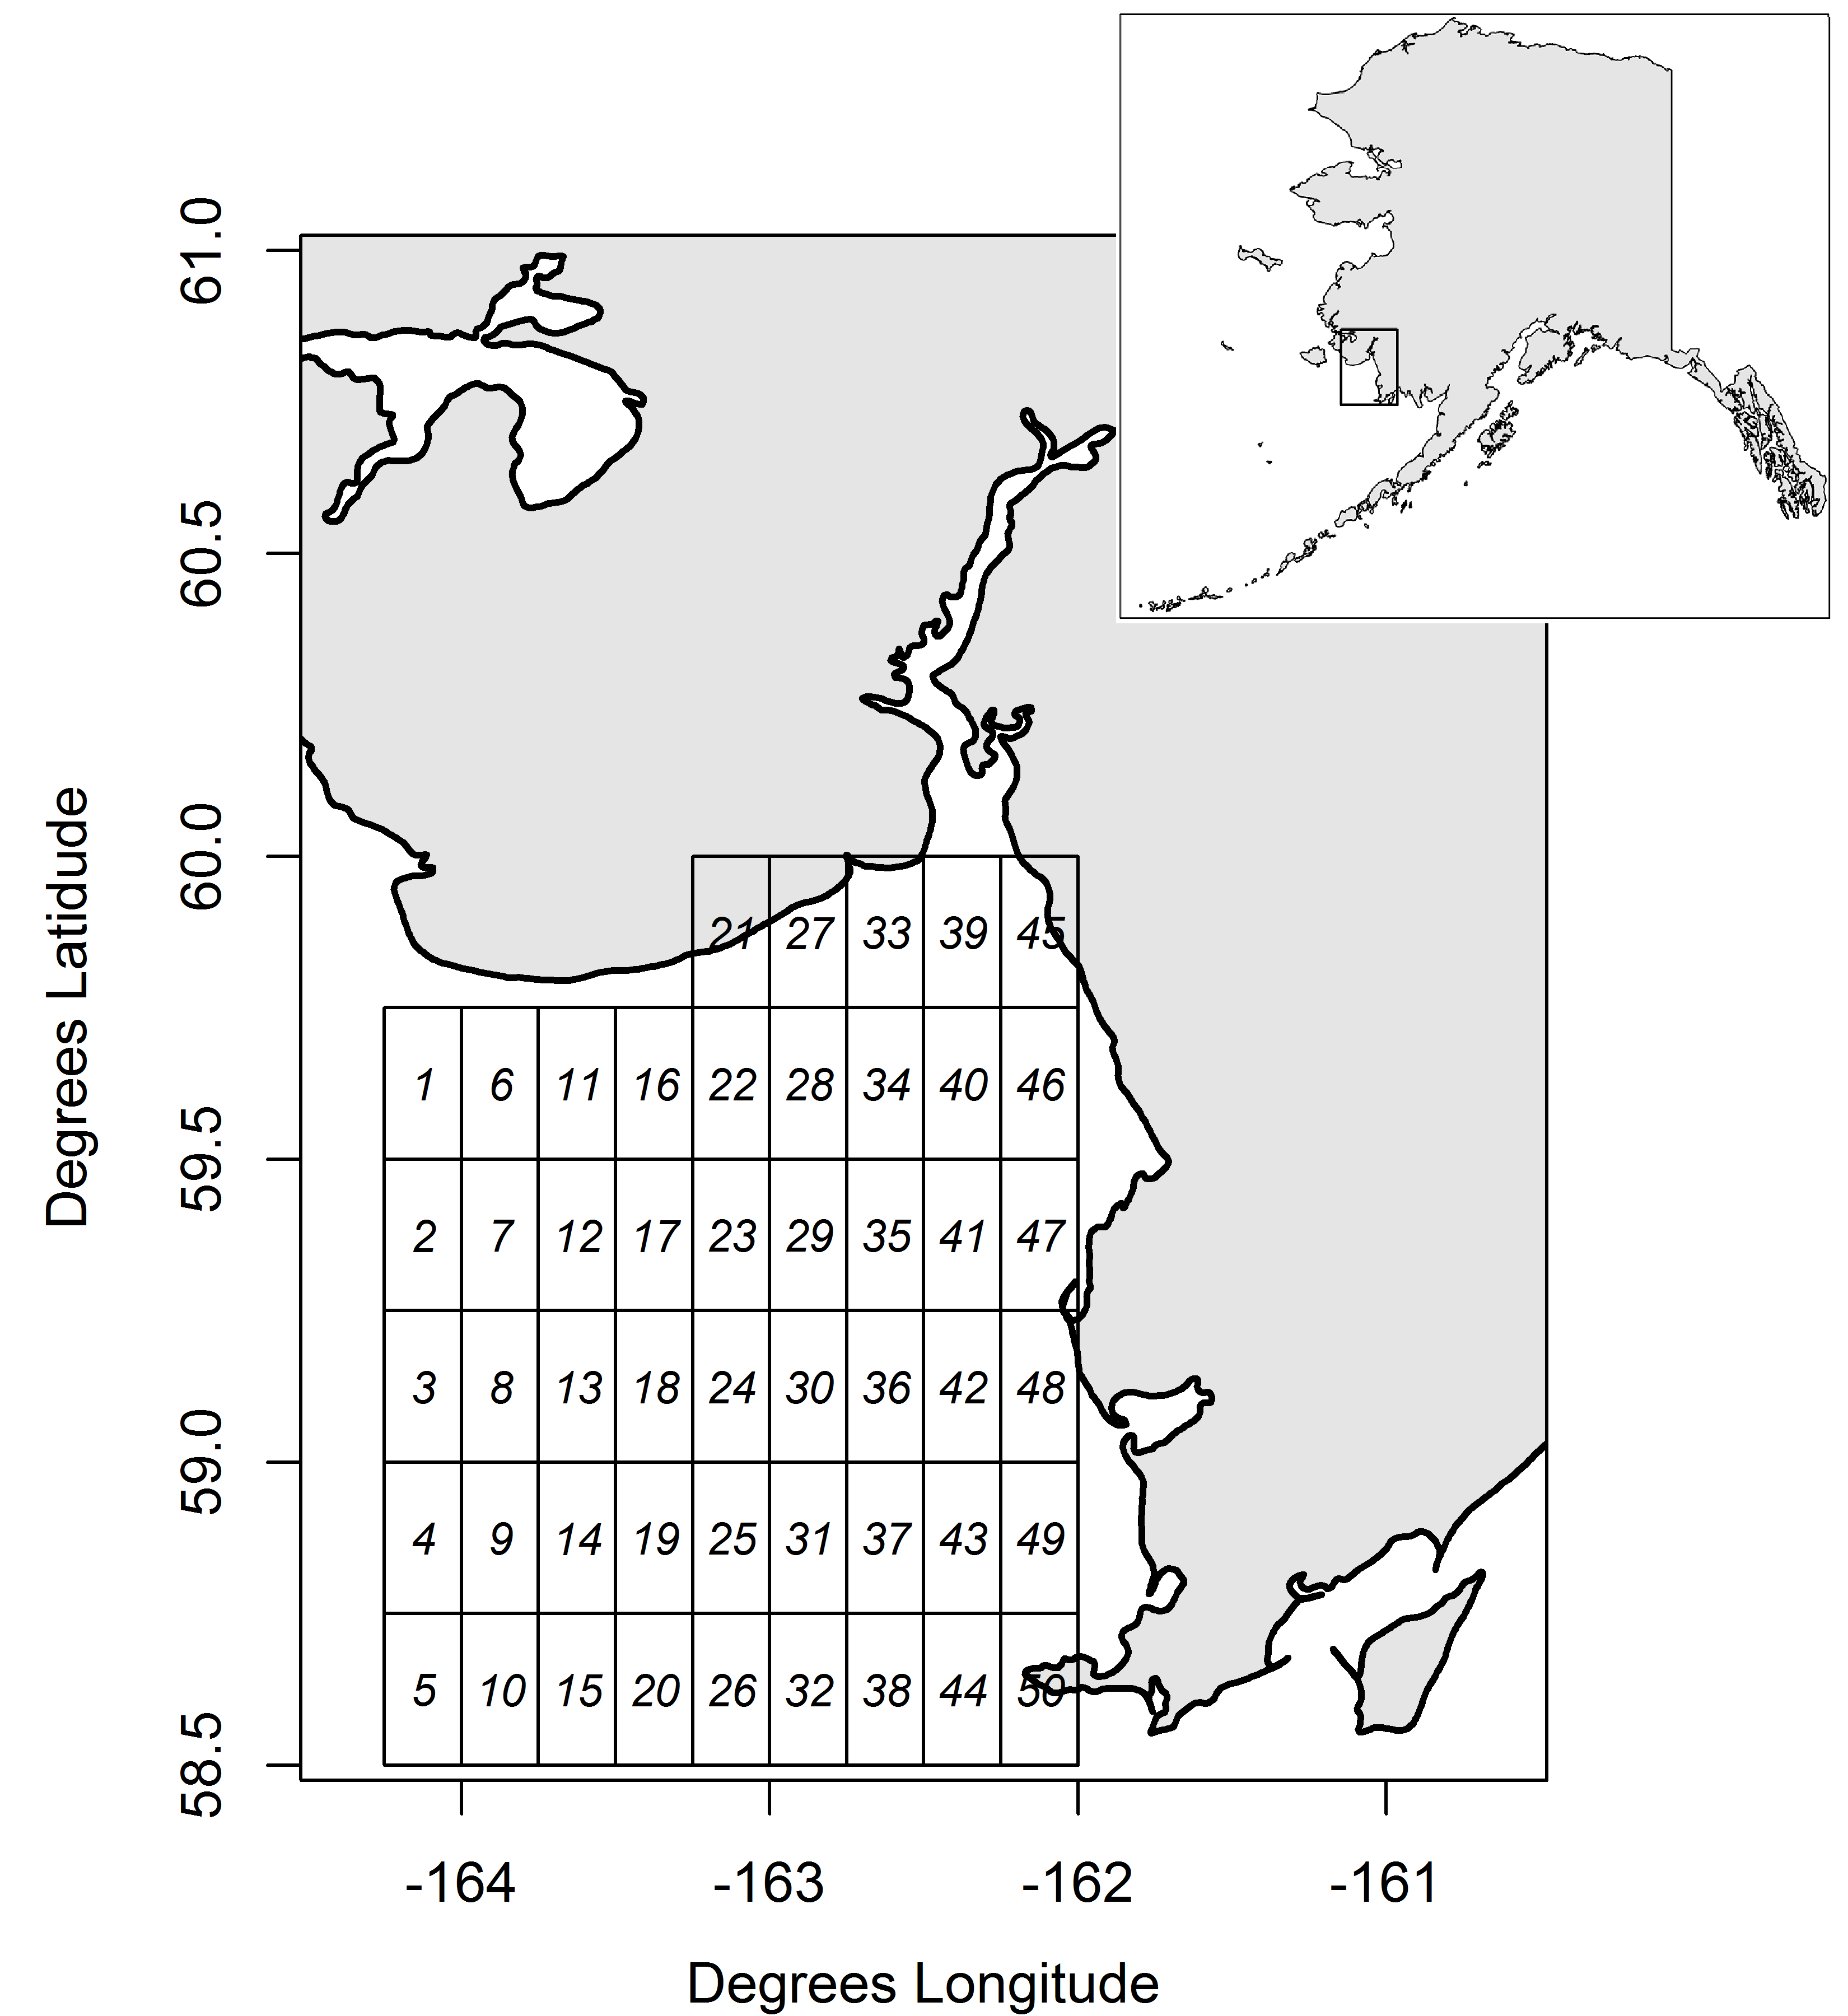
\includegraphics{img/Ch2/map.png}
  \caption{Map of Kuskokwim Bay where Chinook salmon likely stage for transition to freshwater. Shows grid cells from which daily SST values were used. Daily SIC values came from the same grid cells, though excluding grid cell 45 below due to missing values.}
  \label{fig:ch2-map}
\end{figure}

\pagebreak

\begin{figure}
  \centering
  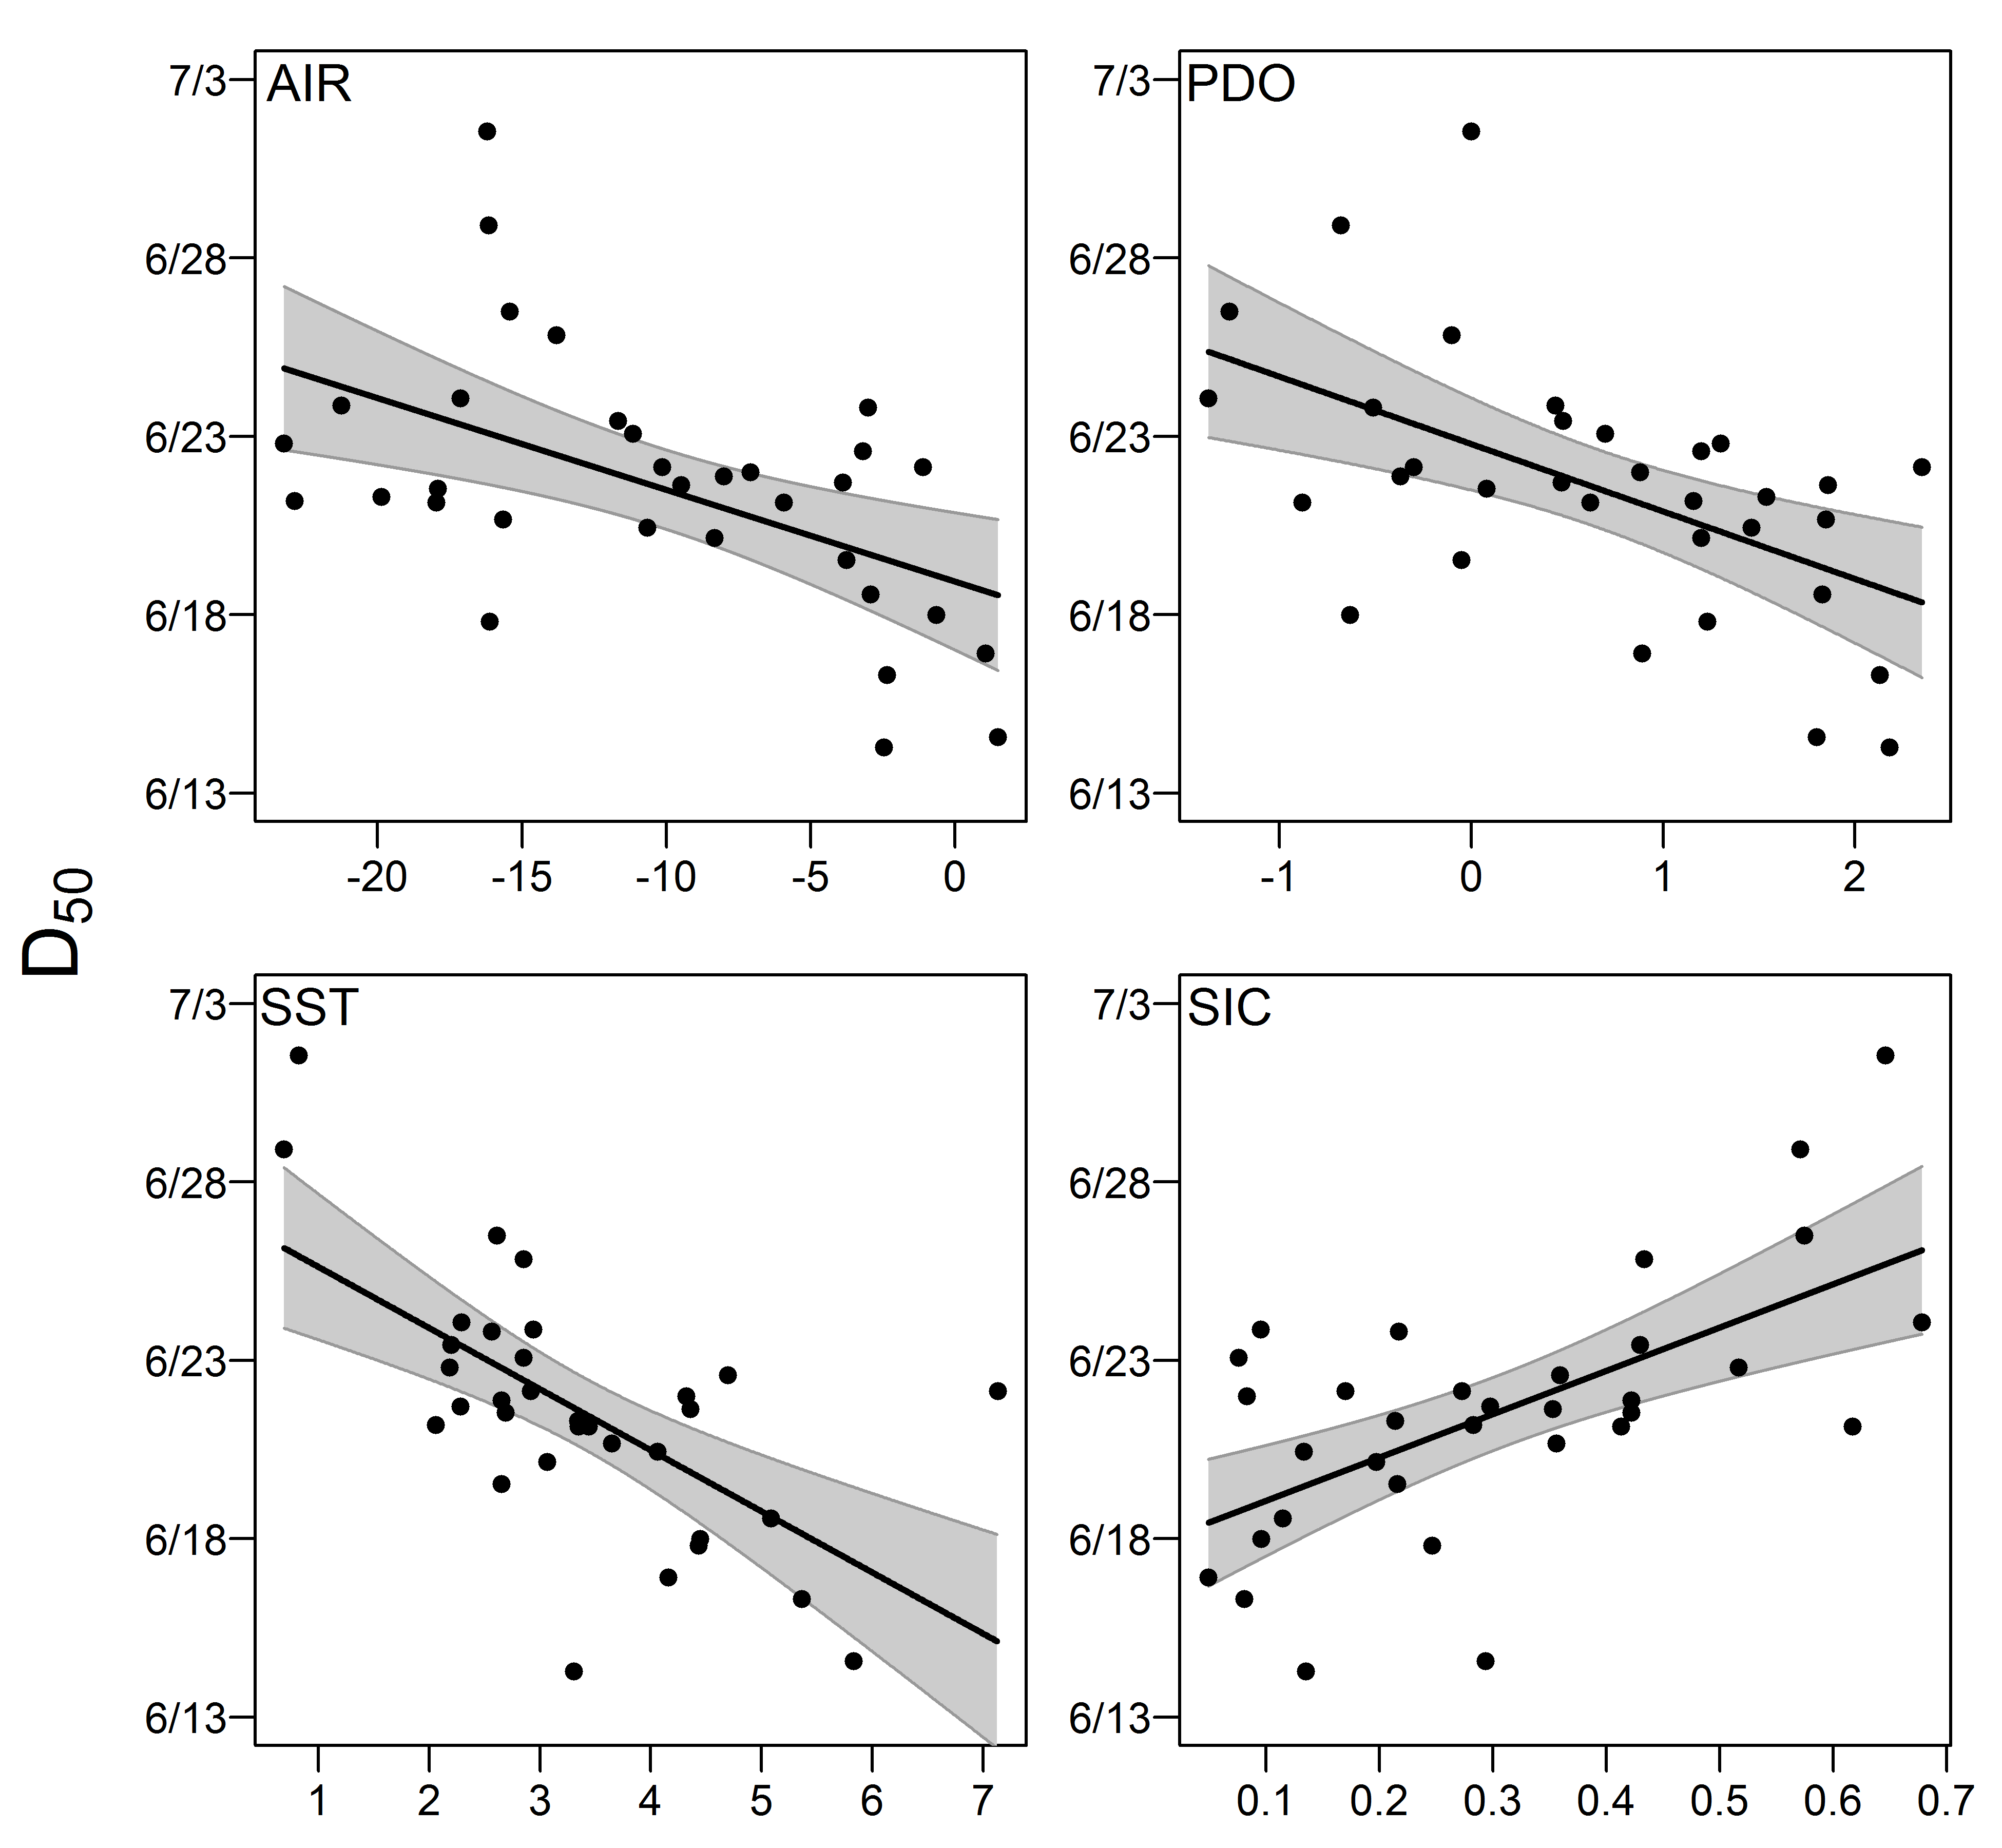
\includegraphics{img/Ch2/relationships.png}
  \caption{Relationships between the four single environmental variables and run timing $\left(D_{50}\right)$ using data from optimal climate windows when 2016 was added to the training data. For illustration purposes only, gridded variables SST and SIC were combined by weighted averaging where the weight of each grid cell was assigned the $\text{AIC}_{\text{c}}$ weight of that grid cell when grid cell-specific models were fit. Grey bands are 95$\%$ confidence intervals on the least squares line.}
  \label{fig:relationships}
\end{figure}

\pagebreak

\begin{figure}
  \centering
  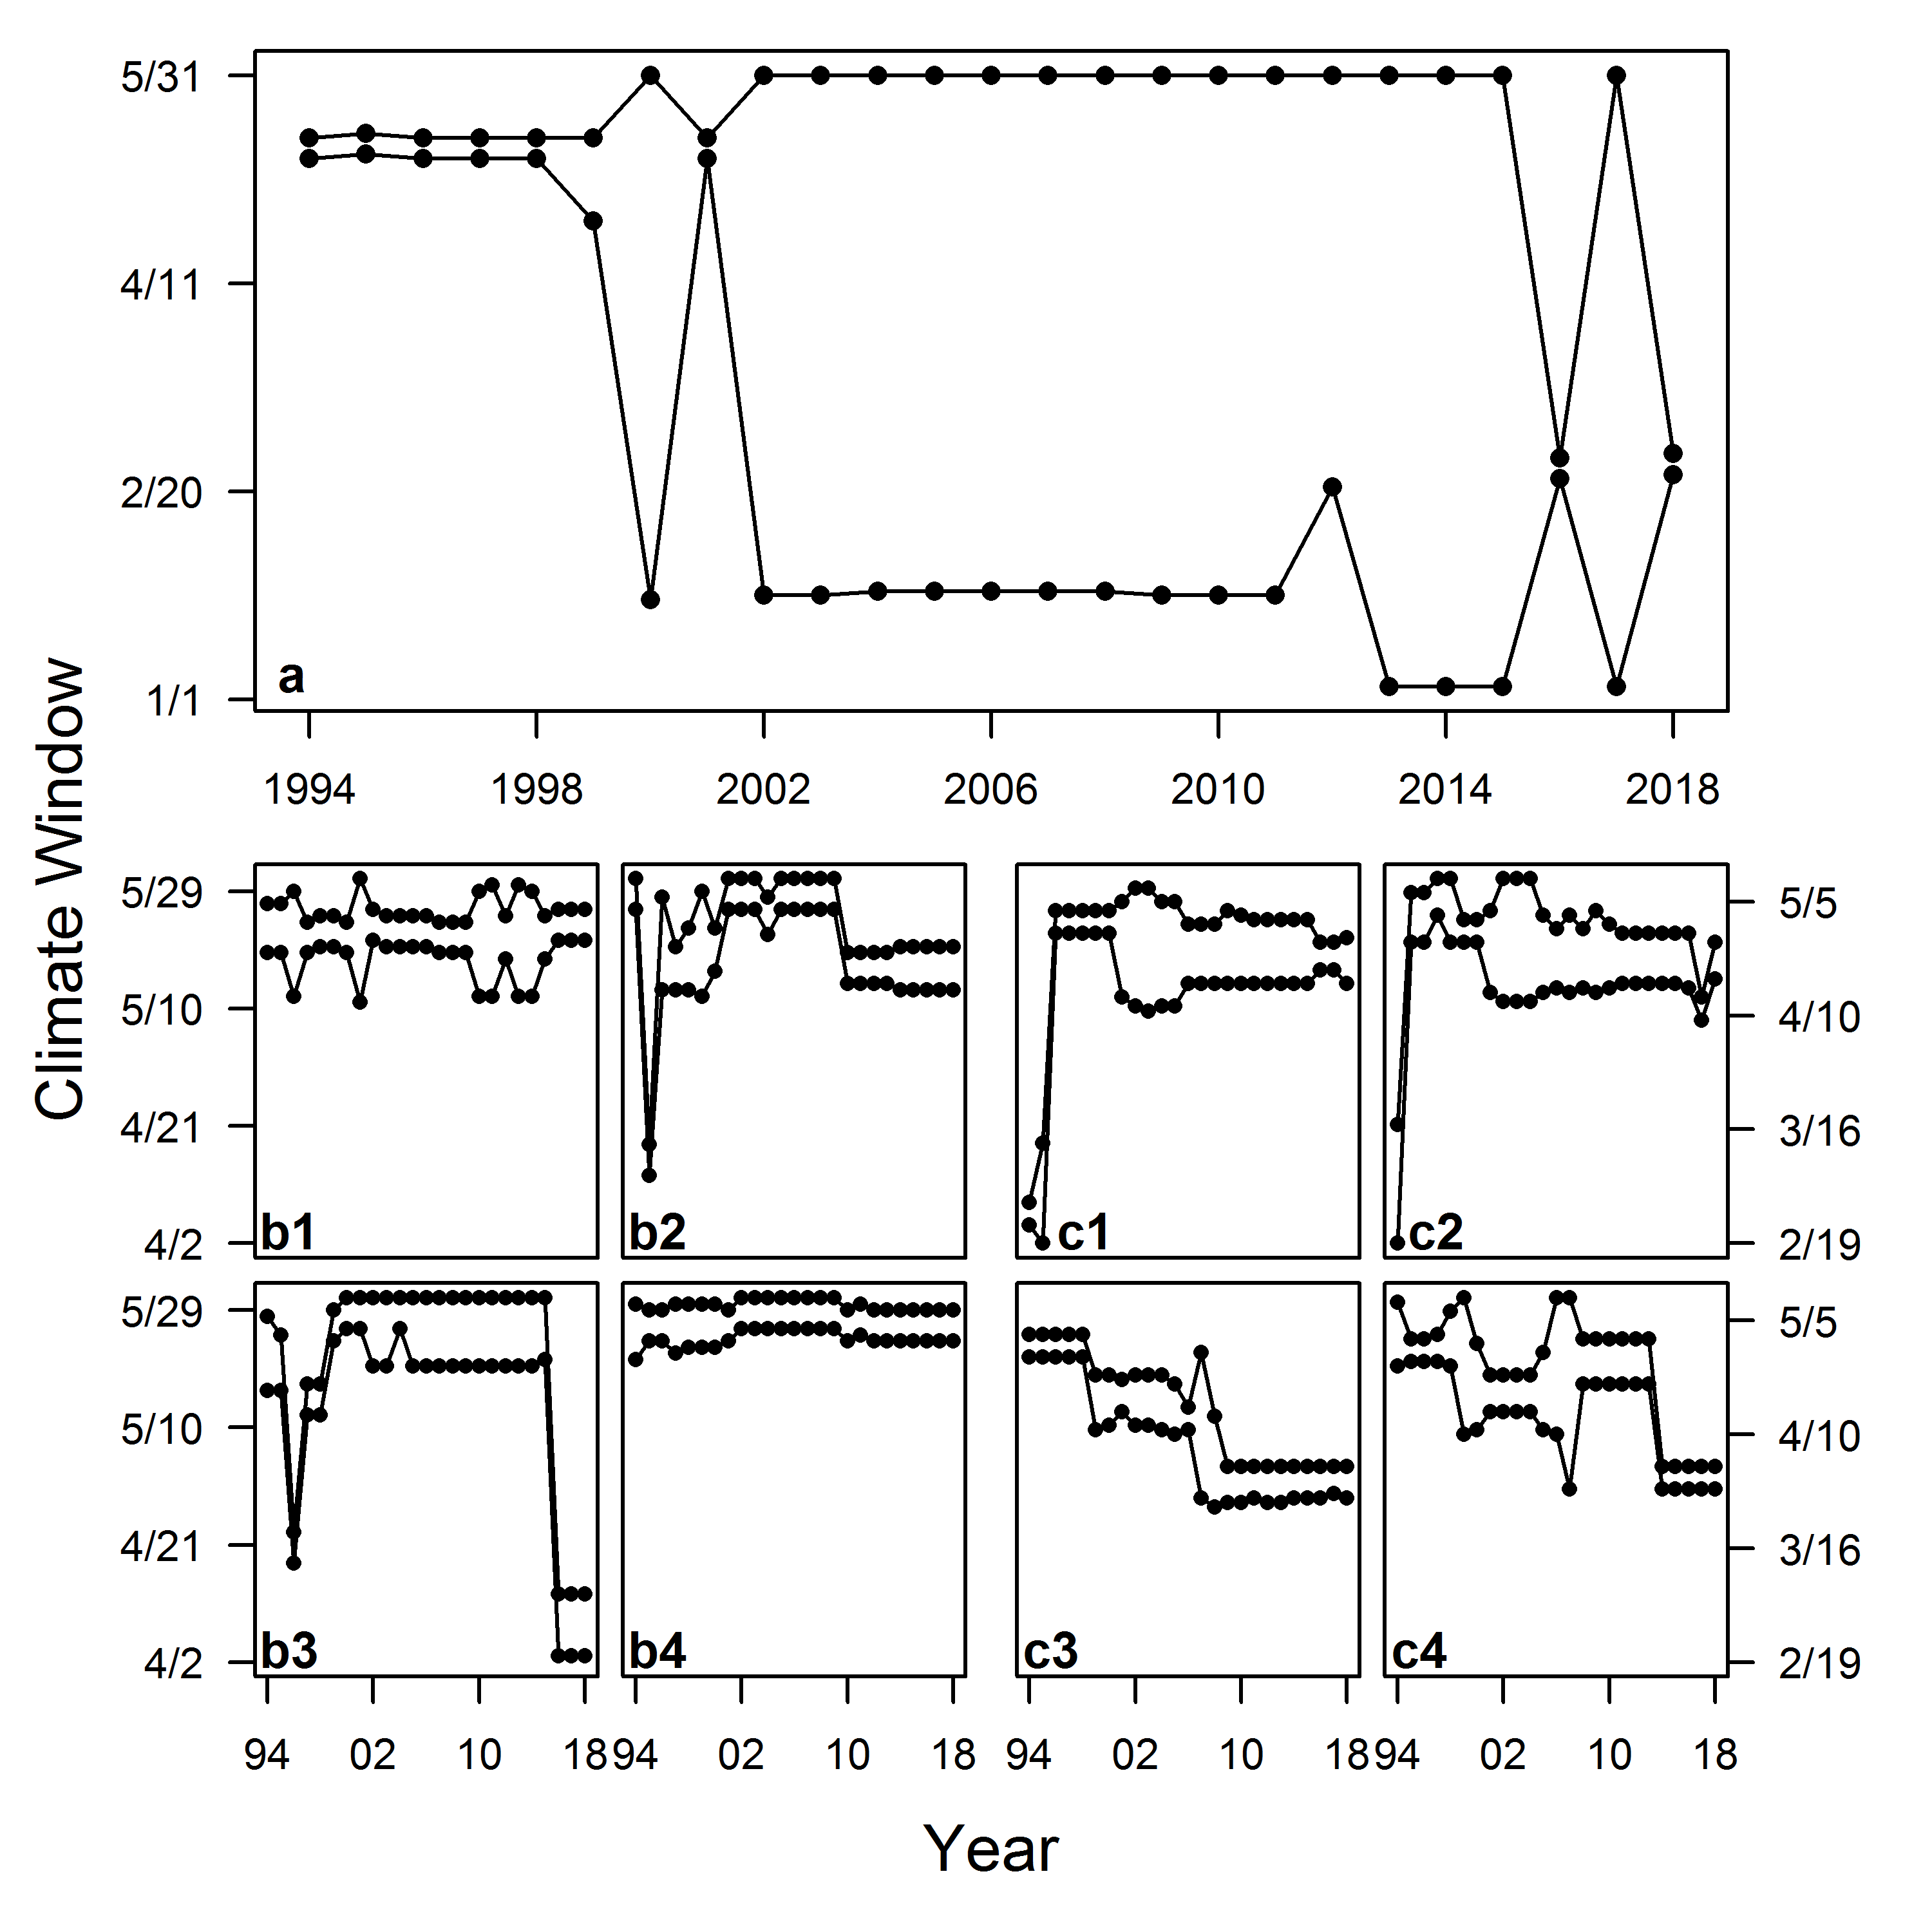
\includegraphics{img/Ch2/window-changes.png}
  \caption{Changes in selected climate windows as training data were added in the retrospective forecasting analysis. Bottom and top lines show the first and last day of the selected climate window, respectively, as more years were added. The year axis corresponds to the selected window after including environmental and run timing data from that year in the training data. E.g., the windows shown for 2015 were used to produce the forecast for 2016. Panel (a) is Bethel air temperature, panels b1-b4 are SST windows for four sample grid cells and panels c1-c4 are SIC windows for the same four sample grid cells. Sample grid cells from Figure \ref{fig:ch2-map} shown for SST and SIC are as follows: grid cell 8 (b1, c1), grid cell 44 (b2, c2), grid cell 12 (b3, c3), and grid cell 48 (b4, c4). Selected windows for PDO are not shown because the single month of May was selected in all years.}
  \label{fig:window-changes}
\end{figure}

\pagebreak

\begin{figure}
  \centering
  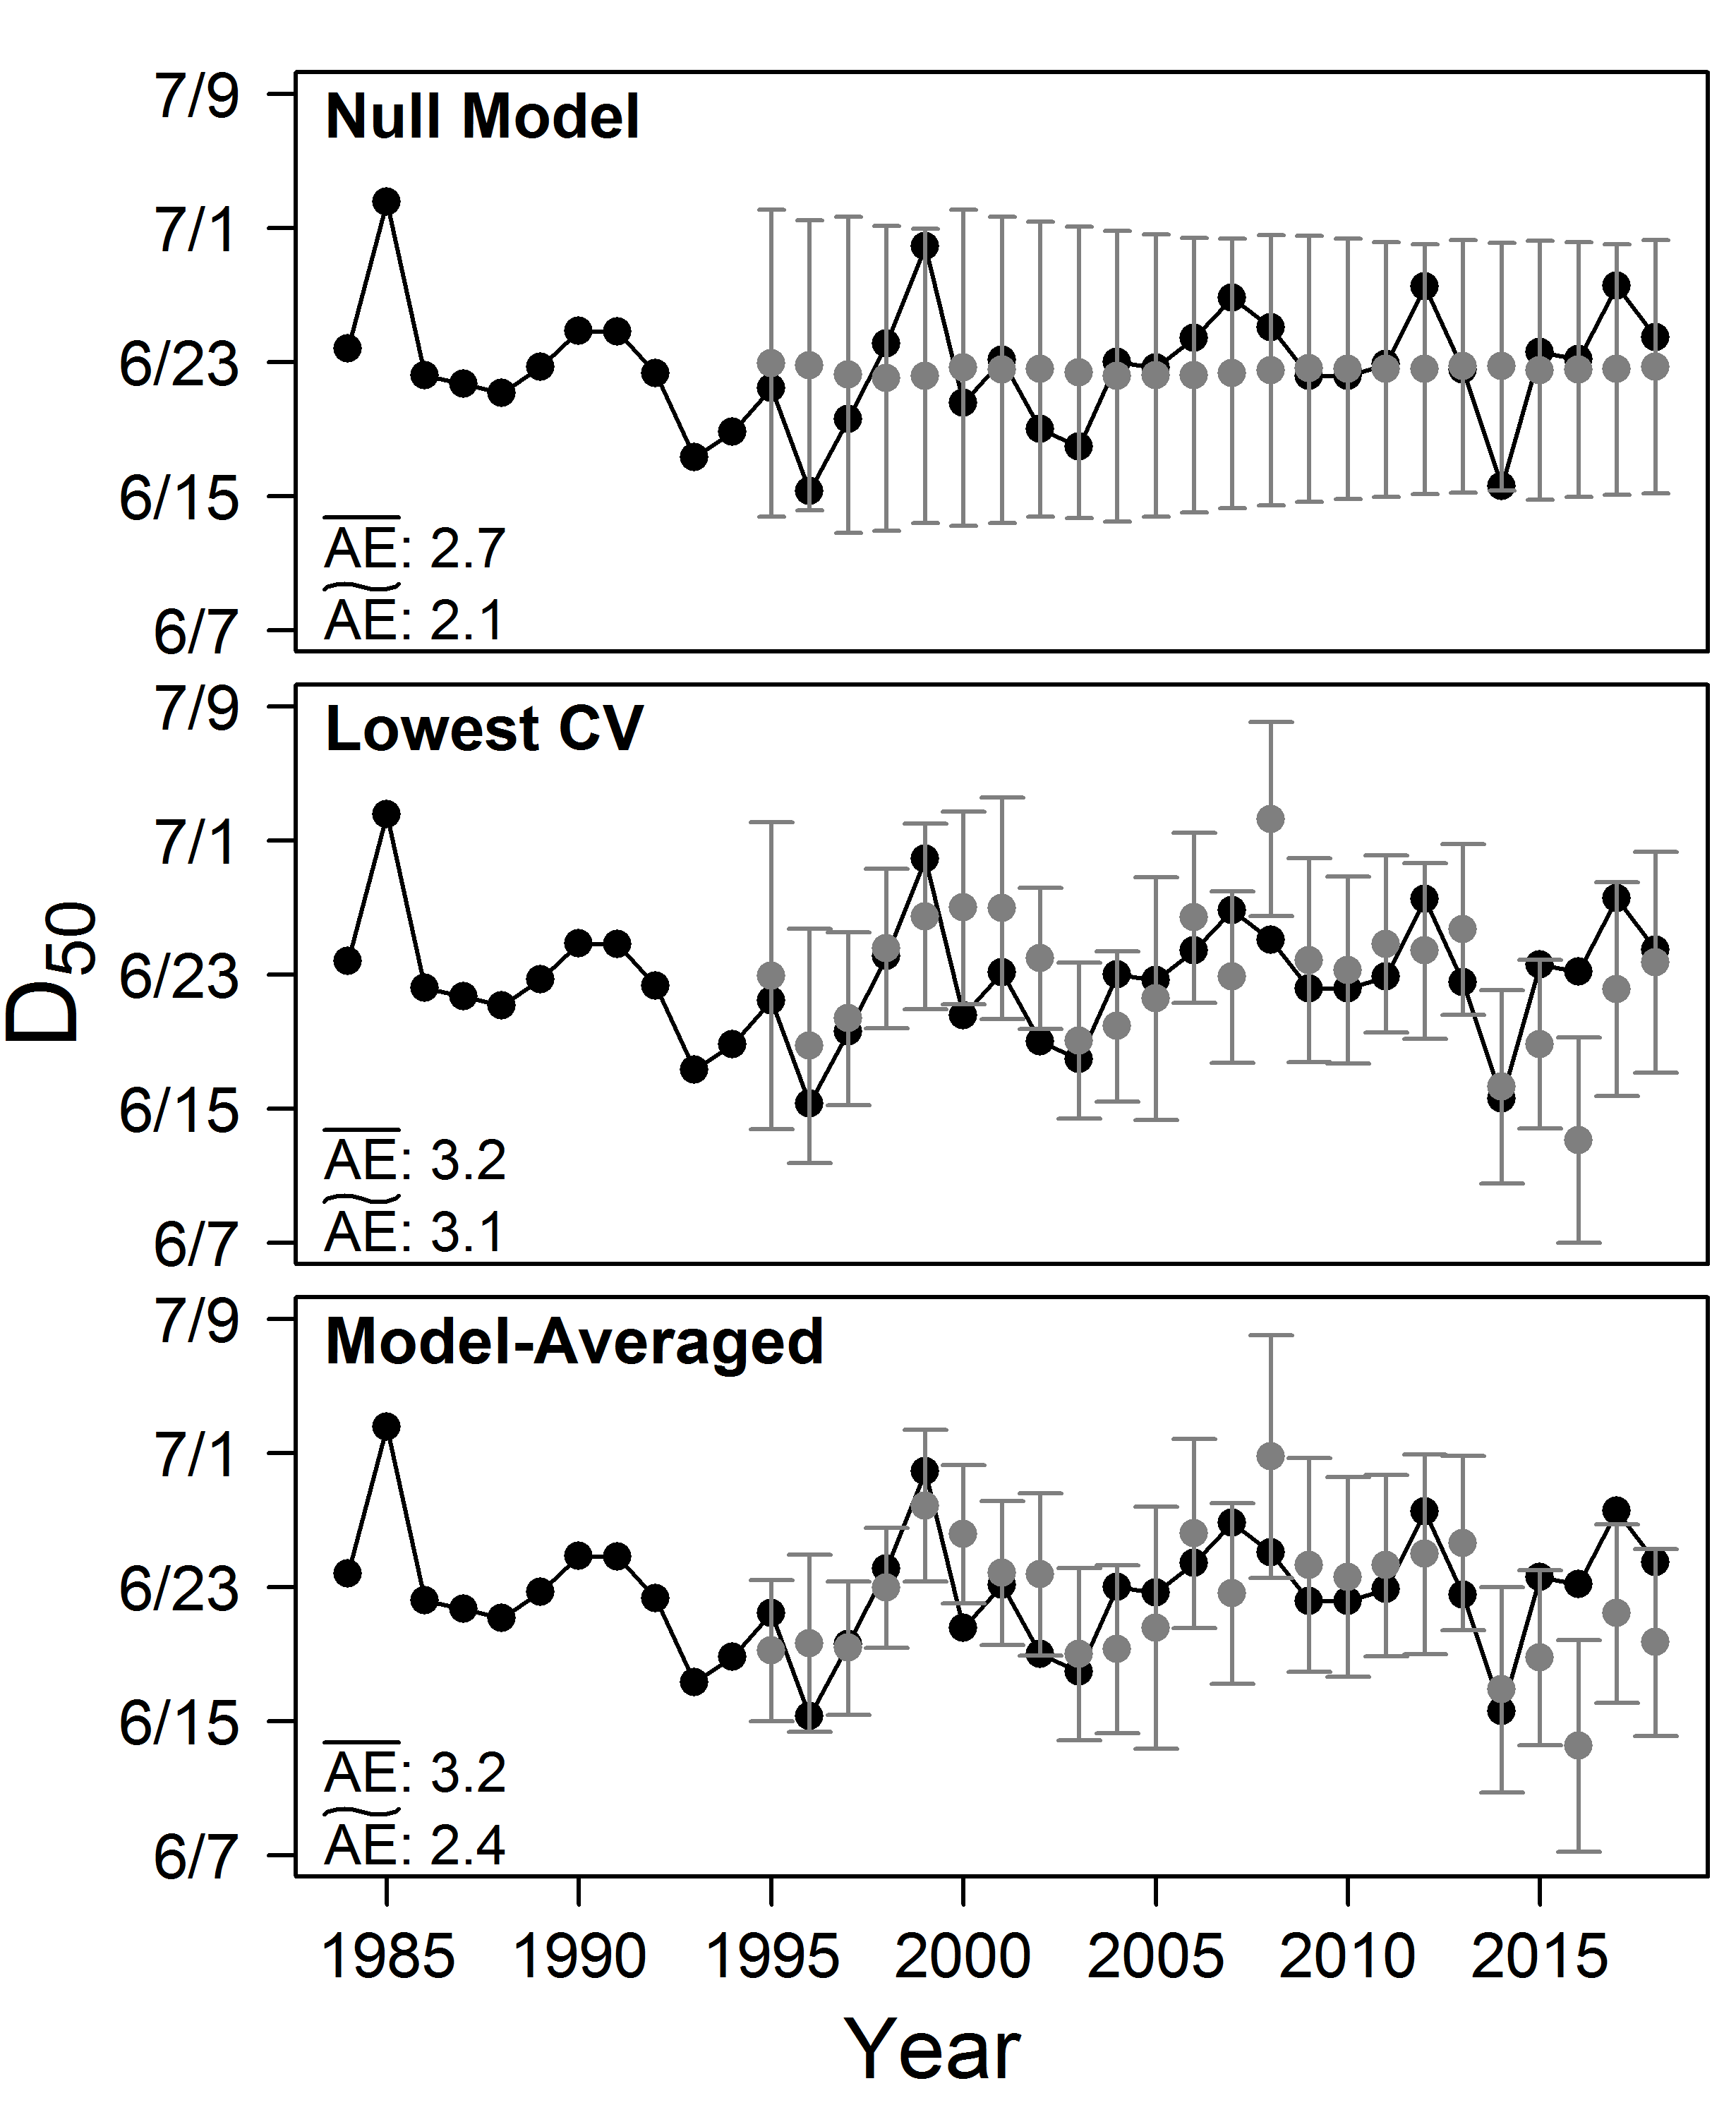
\includegraphics{img/Ch2/forecasts.png}
  \caption{Produced forecasts under the three approaches. Black points/lines are the time series of $D_{50}$ detected by the BTF. Grey points are out-of-sample forecasts with 95$\%$ prediction intervals shown as error bars. $\overline{\text{AE}}$ and $\widetilde{\text{AE}}$ are the mean and median absolute forecast errors from 1995 to 2016, respectively.}
  \label{fig:forecasts}
\end{figure}

\pagebreak

\begin{figure}
  \centering
  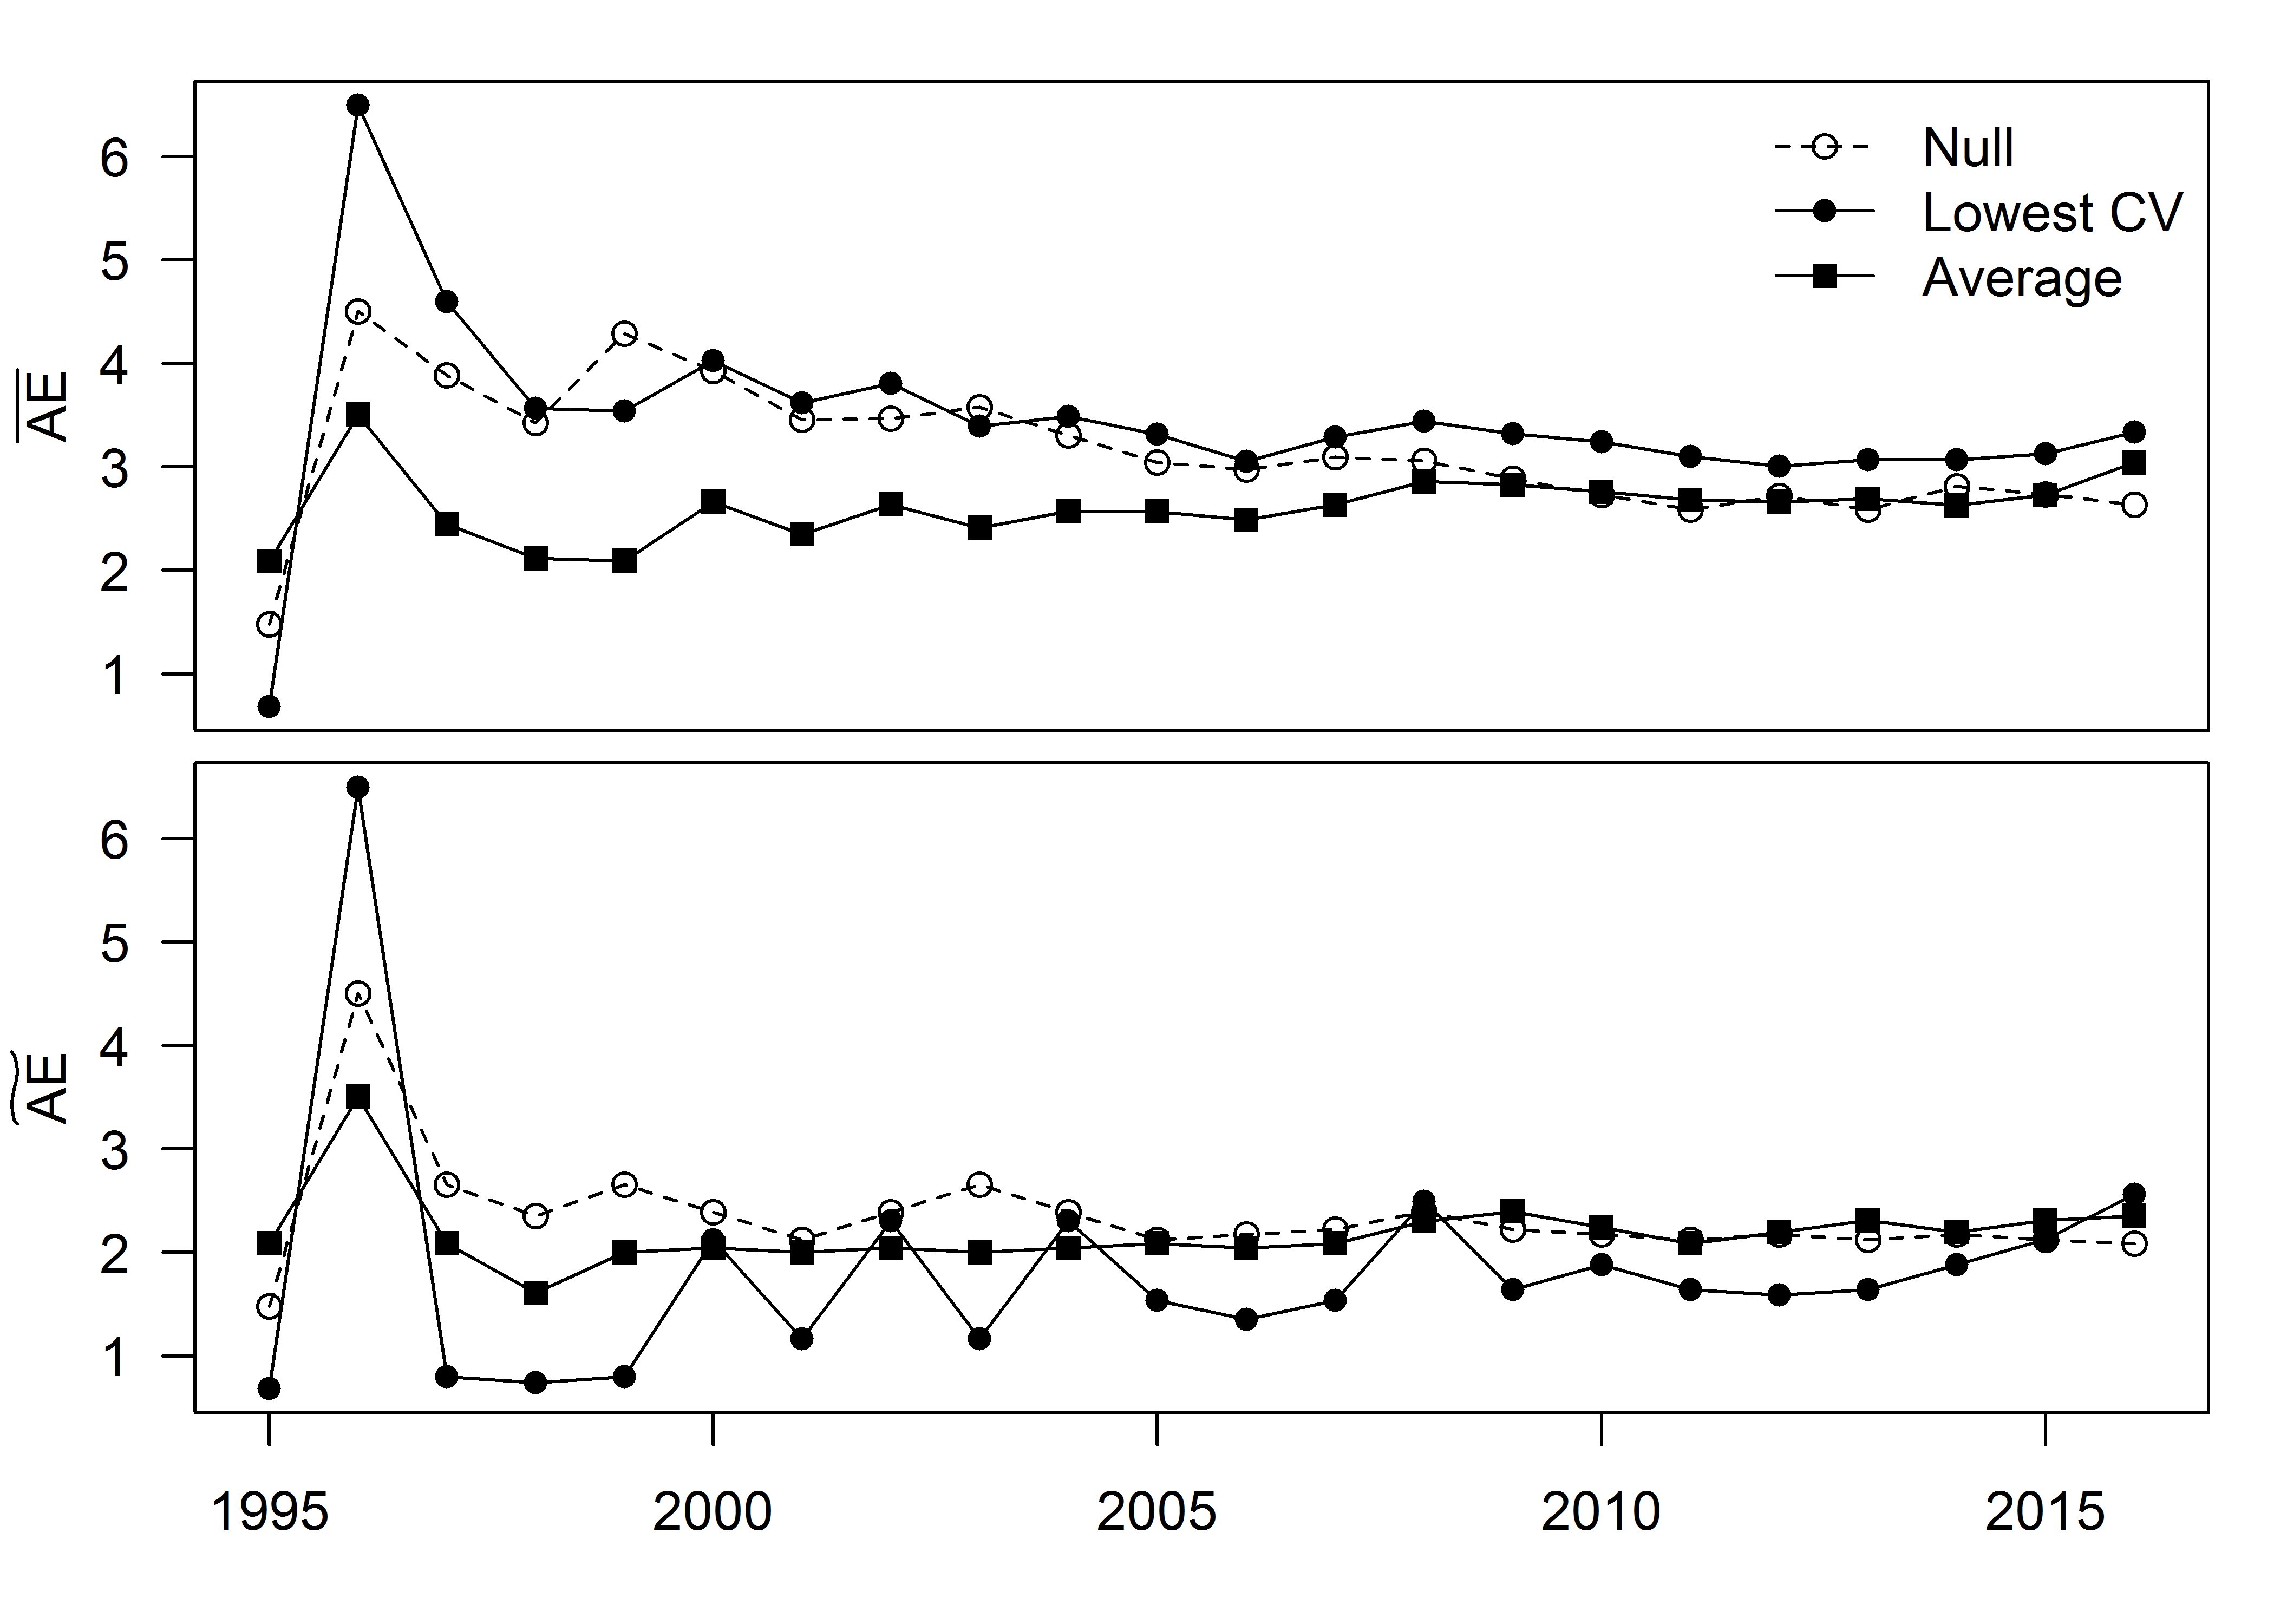
\includegraphics{img/Ch2/ae-changes.png}
  \caption{Evolution of $\overline{\text{AE}}$ (mean) and  $\overline{\text{AE}}$ (median) absolute forecast error under the three investigated forecasting approaches. Each point is the average of absolute errors of all years before and including the corresponding year on the x-axis, starting in 1995.}
  \label{fig:ae-changes}
\end{figure}

\pagebreak

\begin{figure}
  \centering
  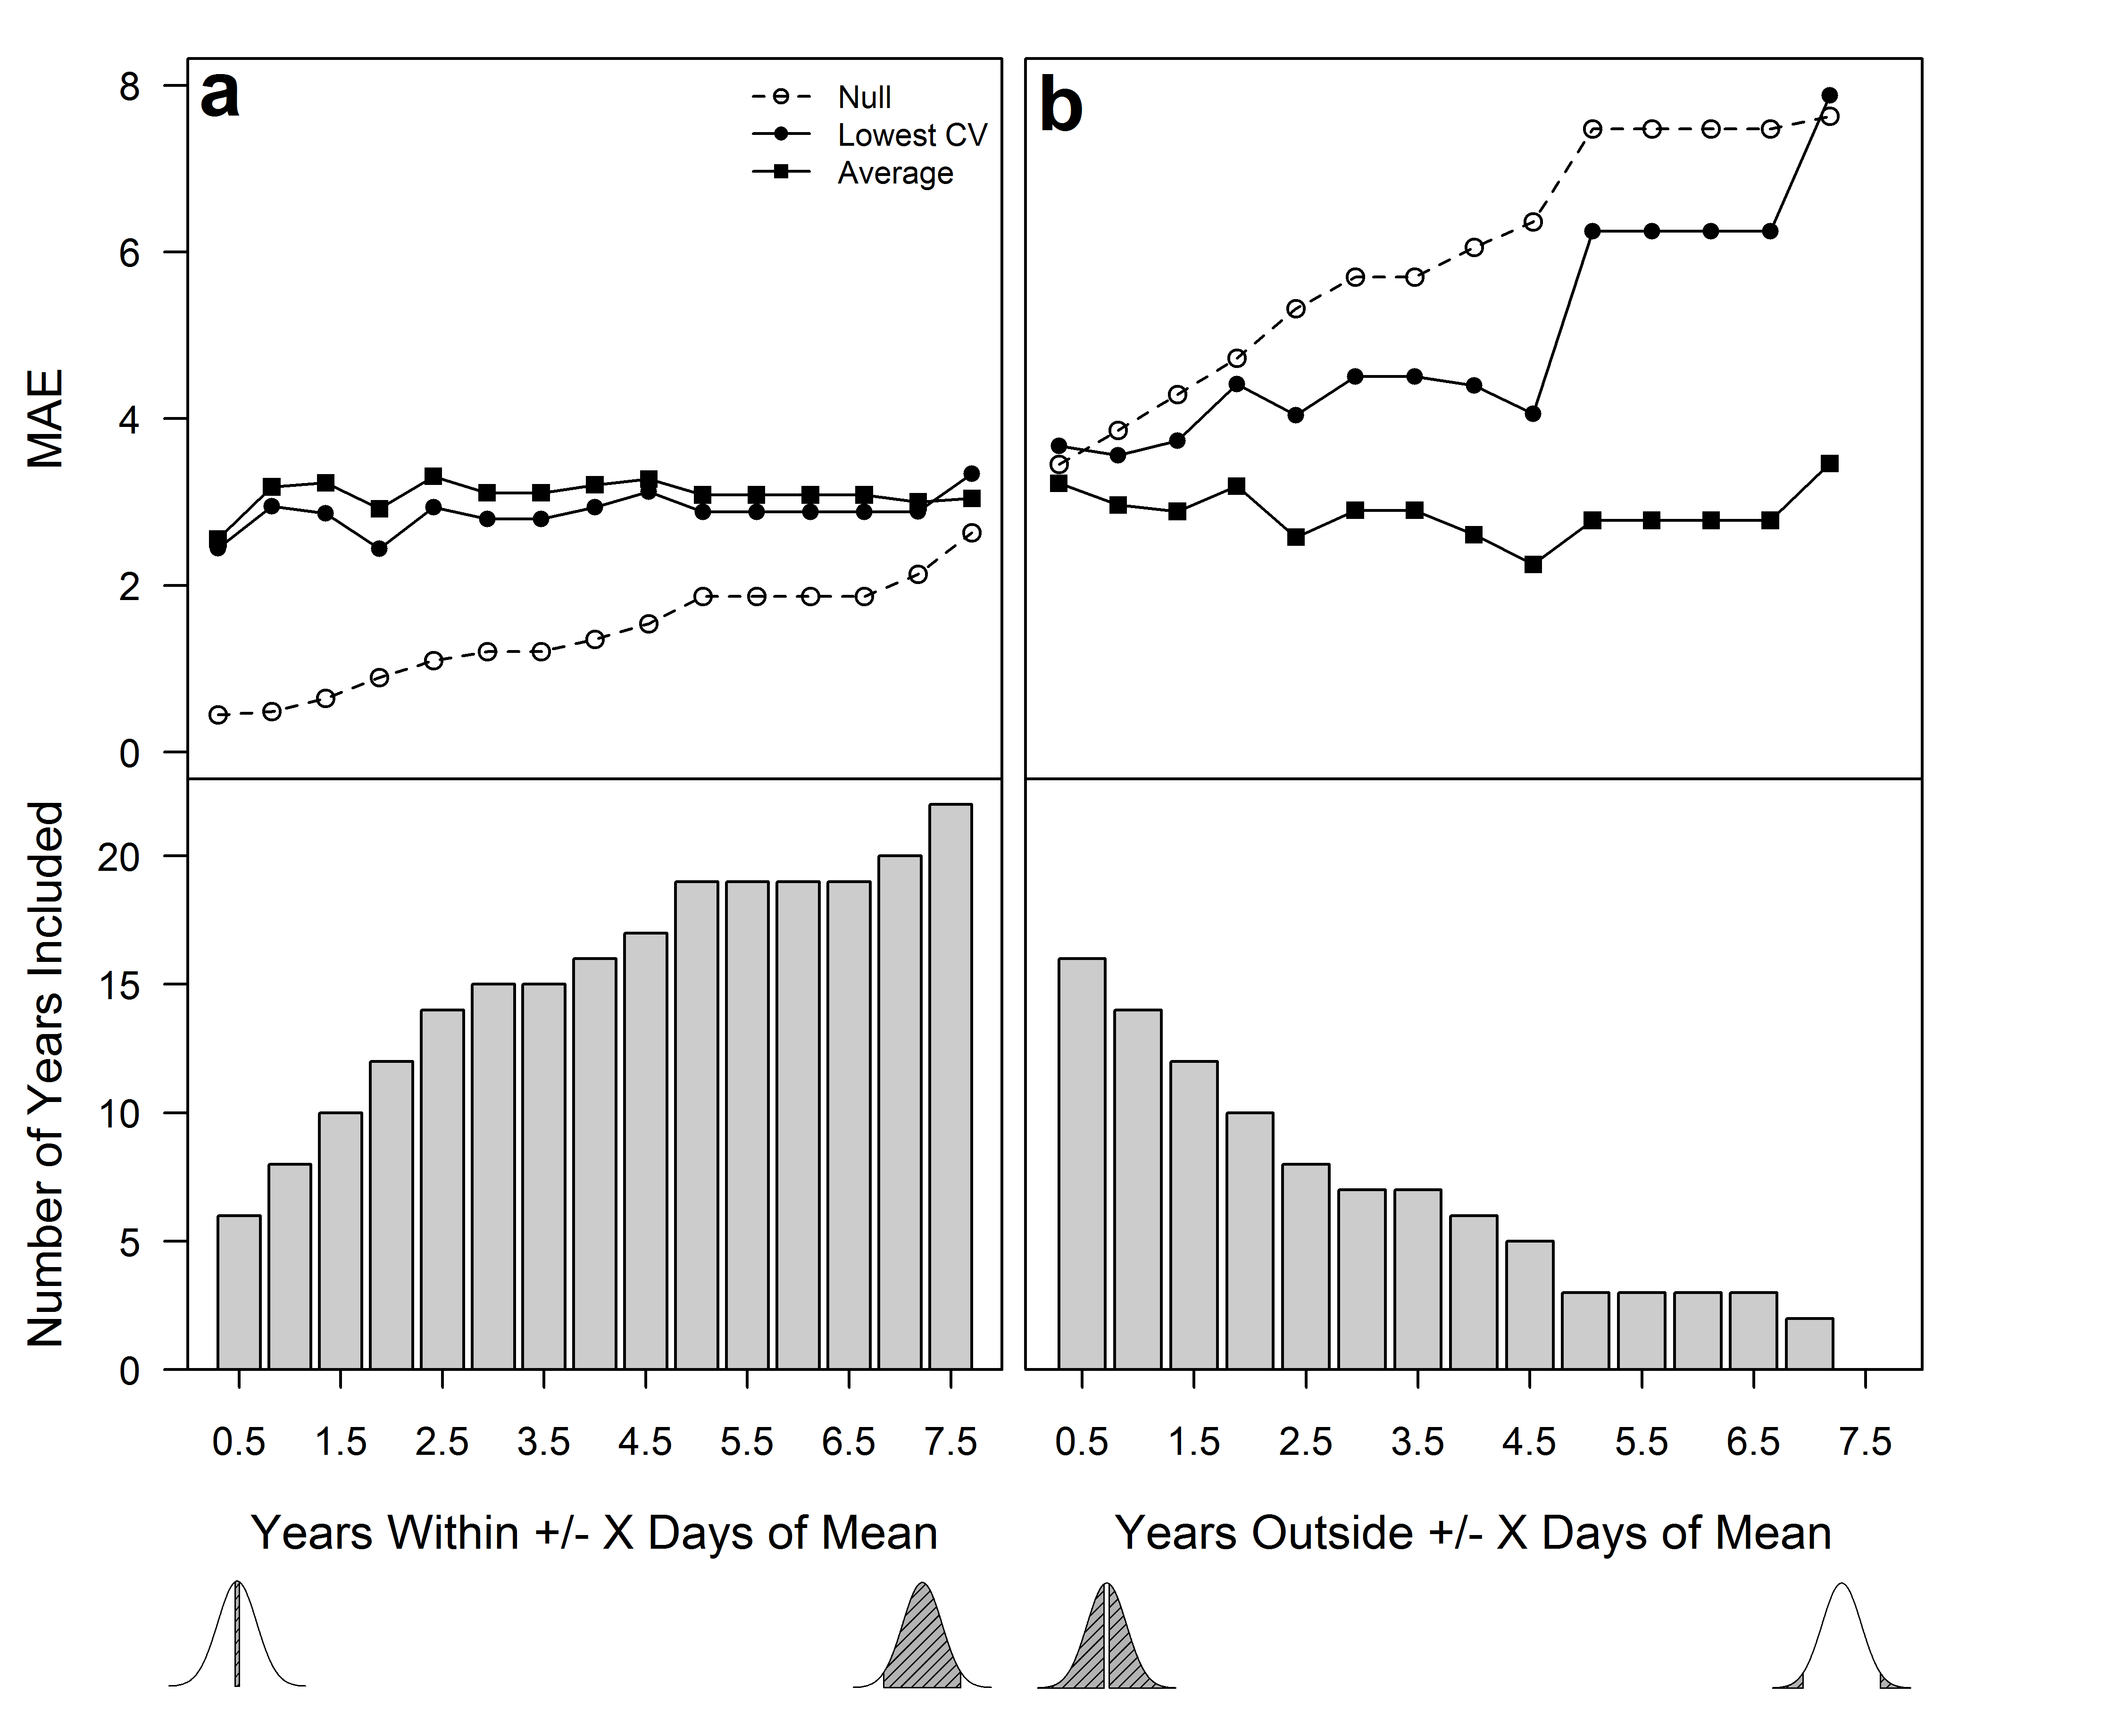
\includegraphics{img/Ch2/mae-subsets.png}
  \caption{$\overline{\text{AE}}$ under three forecast approaches calculated by either (a) including years with a $D_{50}$ value within $\pm x$  days of the all-year average or (b) including years with a $D_{50}$ value outside $\pm x$ days of average, where $x$ is the number of days indicated on the $x$-axis. Bottom panels show the number of observed years in which the appropriate $\pm x$ days criterion was met. Shaded regions in the hypothetical distributions show the types of $D_{50}$ values that were included in the calculation of $\overline{\text{AE}}$. One point that may enrich inference from this figure (and is shown in the shaded normal distributions) is that panel (a) becomes more inclusive from left to right by adding years that are more dissimilar to the average in the calculation of $\overline{\text{AE}}$ whereas panel (b) becomes more exclusive from left to right by removing years that are similar to the average.}
  \label{fig:mae-subsets}
\end{figure}

\pagebreak

\begin{figure}
  \centering
  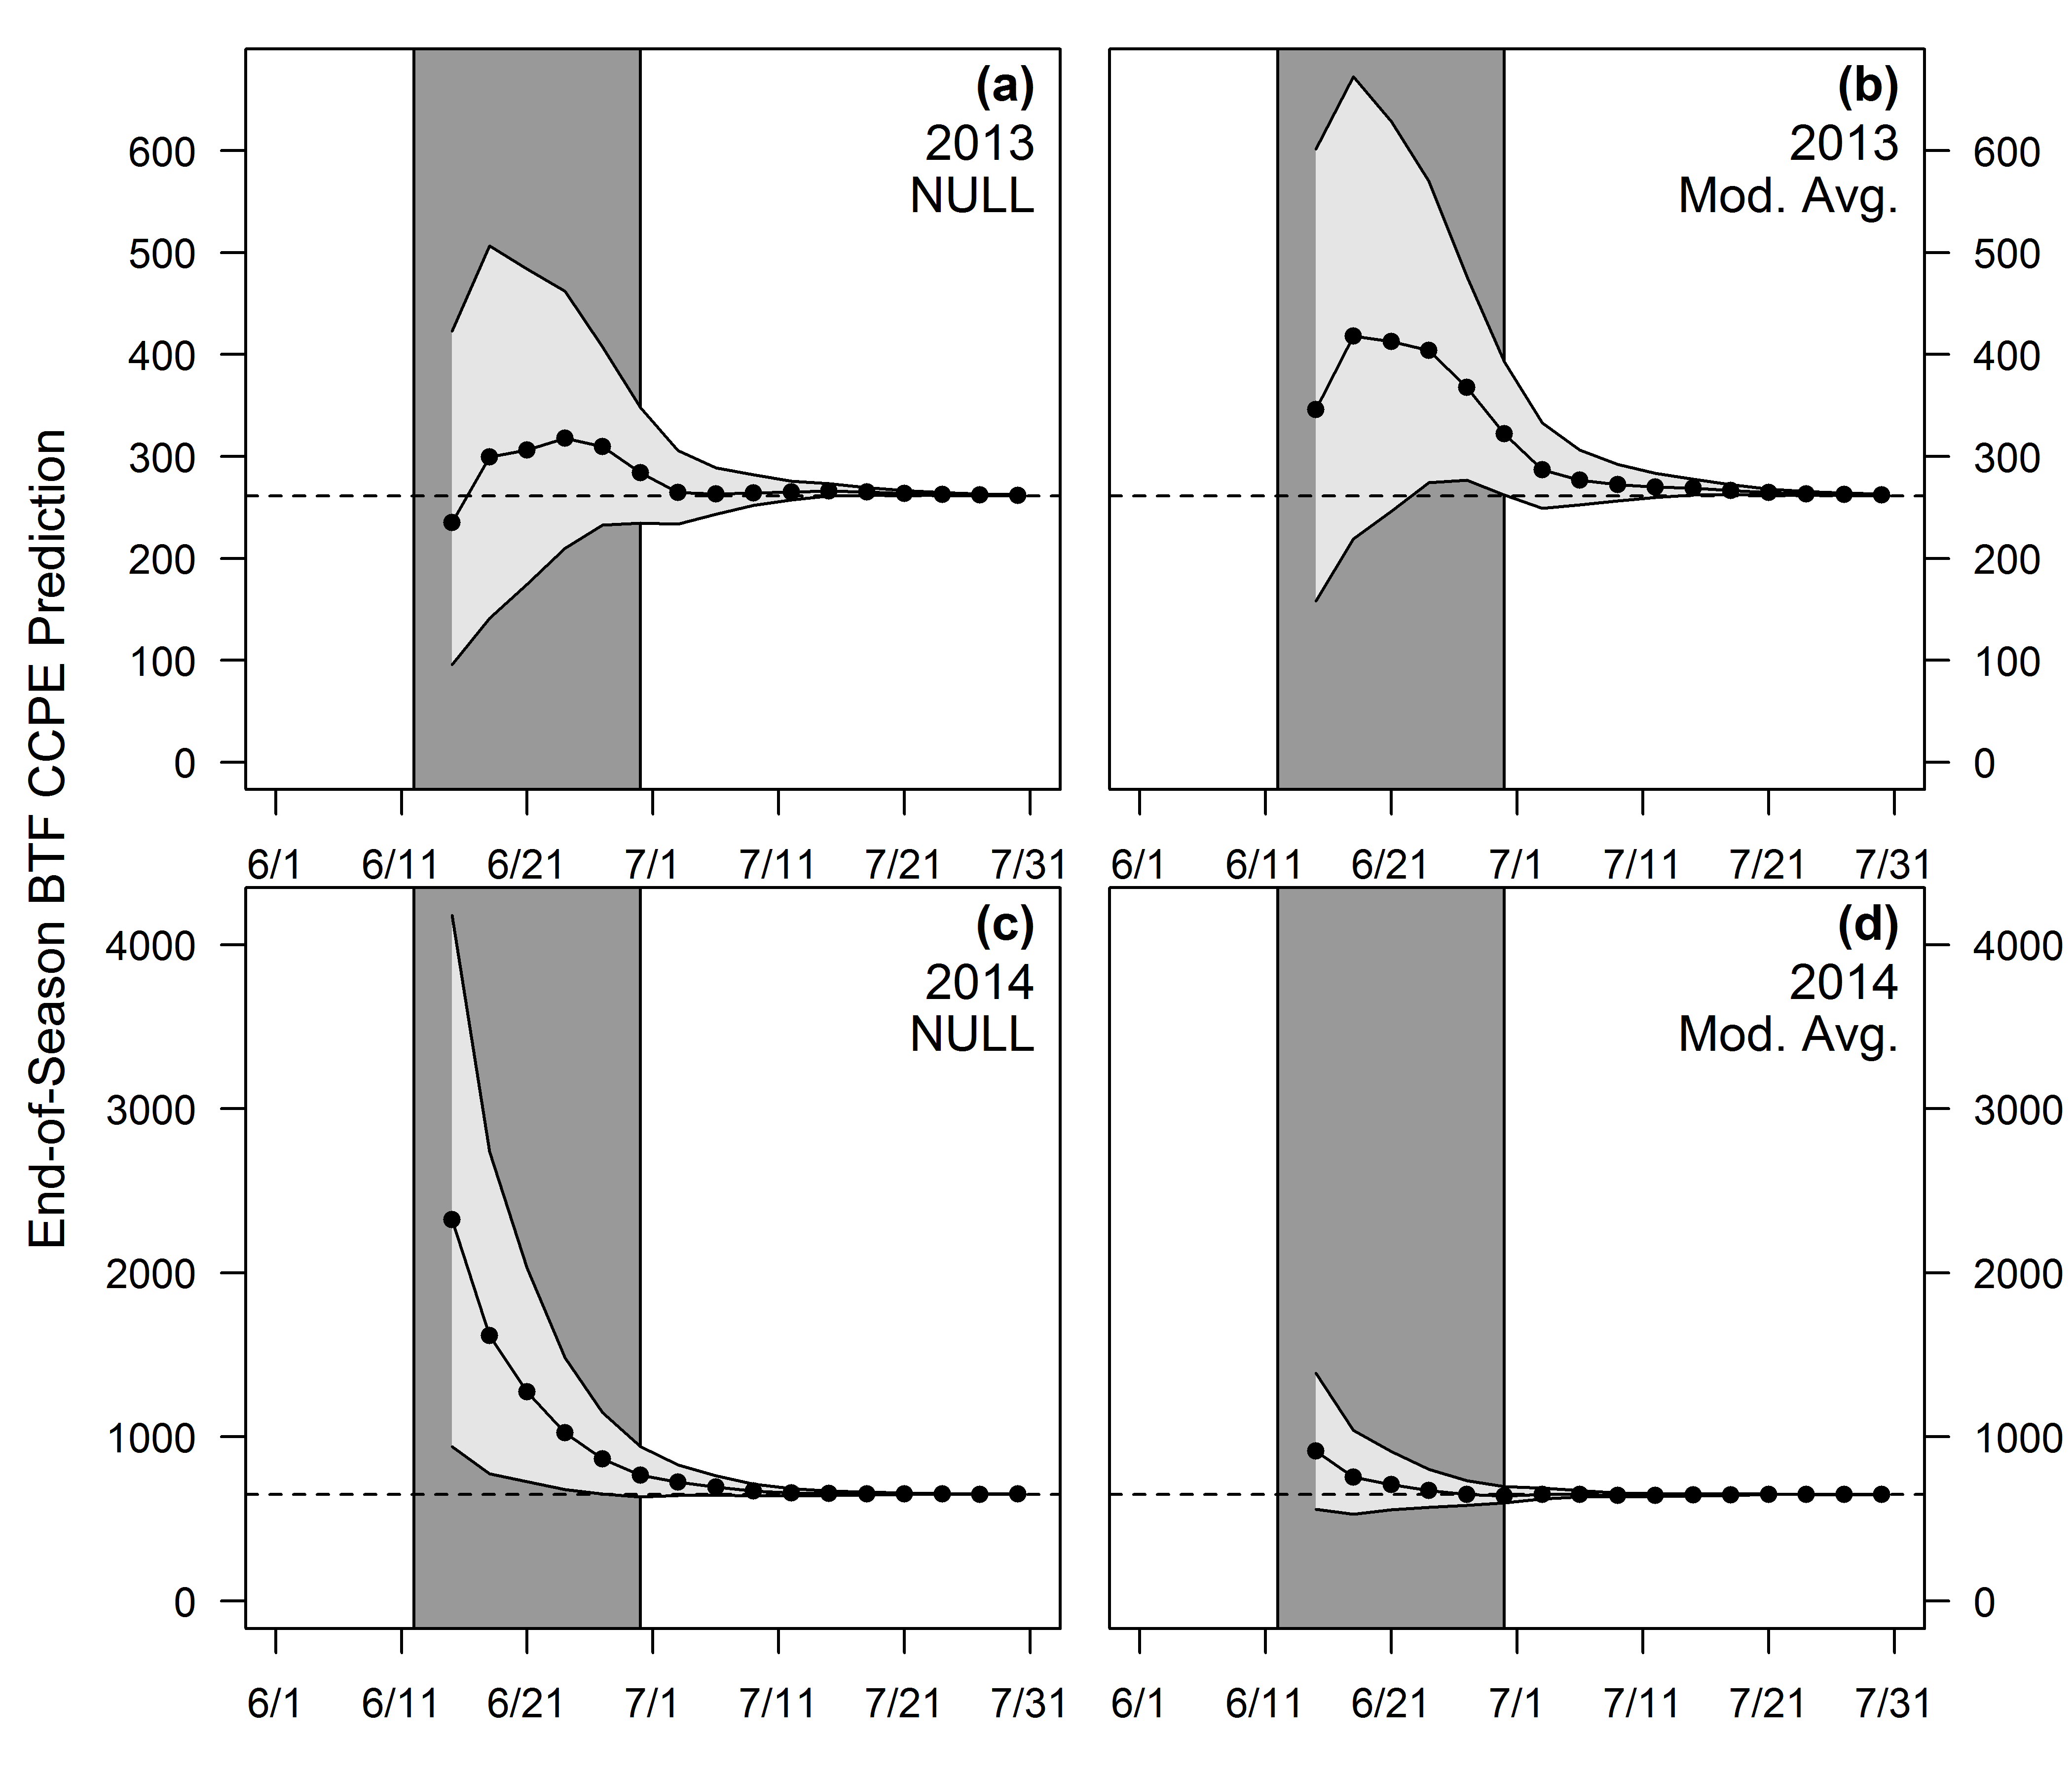
\includegraphics{img/Ch2/eos-preds.png}
  \caption{In-season predictions of end of season cumulative BTF CPUE under the model-averaged forecast using environmental variables and the forecast under the null model in 2013 and 2014. Intended to illustrate cases in which a manager would benefit from having access to the model-averaged run timing forecast model using environmental variables (2014) and when the null model would have performed better (2013). Horizontal lines are the true end of season cumulative BTF CPUE, dark grey regions are 50$\%$ confidence intervals, and light grey regions are 95$\%$ confidence intervals. Grey vertical lines indicate the period when key harvest decisions are made.}
  \label{fig:eos-preds}
\end{figure}

\chapter{Evaluation of Intra-Annual Harvest Control Rules via
Closed-Loop Simulation}\label{ch3}

\section{Introduction}\label{introduction-1}

Here's chapter 3. It's about in-season simulation models for management
strategy evaluations.

\section{Methods}\label{methods-1}

I did some stuff.

\section{Results}\label{results-1}

I found some stuff.

\section{Discussion}\label{discussion-1}

Here's what it means.

\emph{Insert Tables}

\emph{Insert Figures}

\chapter{Simulation-based Evaluation of Assessment Approaches for
Mixed-stock Pacific Salmon Fisheries}\label{ch4}

\section{Introduction}\label{introduction-2}

Here's chapter 4. It's about different ways to estimate the biological
reference points for a salmon system made up of multiple substocks with
heterogeneity in size and productivity.

\section{Methods}\label{methods-2}

I did some stuff.

\section{Results}\label{results-2}

I found some stuff.

\section{Discussion}\label{discussion-2}

Here's what it means.

\emph{Insert Tables}

\emph{Insert Figures}

\chapter{Conclusions}\label{ch5}

This chapter contains my thoughts on the topic of the dissertation. What
was found, what will be useful to use in the future, what should be
looked at in more detail?

\hypertarget{appendix-a}{\chapter*{Appendix A}\label{appendix-a}}
\addcontentsline{toc}{chapter}{Appendix A}

\noindent
This appendix contains the necessary code to perform two of the main
parts of the run timing forecast model approach in Chapter \ref{ch2}.

\section*{Forecast Cross-Validation}\label{forecast-cross-validation}
\addcontentsline{toc}{section}{Forecast Cross-Validation}

\subsubsection*{Function Name}\label{function-name}
\addcontentsline{toc}{subsubsection}{Function Name}

\texttt{forecast.CV}

\subsubsection*{Purpose}\label{purpose}
\addcontentsline{toc}{subsubsection}{Purpose}

\subsubsection*{Arguments}\label{arguments}
\addcontentsline{toc}{subsubsection}{Arguments}

\noindent
\textbf{Arguments:}

\begin{enumerate}
\def\labelenumi{\arabic{enumi}.}
\tightlist
\item
  \texttt{x}: a vector containing the time series of the x-variable
\item
  \texttt{y}: a vector containing the time series of the y-variable
\item
  \texttt{start.ind}: the index to start the forecast cross-validation
  (e.g., 10 would train to 10 years and start forecasting in the
  \(11^{\text{th}}\), then continue until present).
\item
  \texttt{na.rm}: logical; do you wish to remove \texttt{NA}
  observations before calculating summary statistics?
\item
  \texttt{include.last.year.in.scores}: logical; do you wish to have the
  last year of \texttt{y} to influence the cross-validation score?
\end{enumerate}

\subsubsection*{Psuedocode}\label{psuedocode}
\addcontentsline{toc}{subsubsection}{Psuedocode}

\subsubsection*{Source Code}\label{source-code}
\addcontentsline{toc}{subsubsection}{Source Code}

\begin{verbatim}
forecast.CV = function(x, y, start.ind, na.rm = F, include.last.year.in.scores = T) {  
  # total number of observed pairs
  n = length(x)
  # validation end years
  val.end = start.ind:(n-1)
  n.val = length(val.end)
  # containers
  error = numeric(n.val)
  abs.error = numeric(n.val)
  pred.se = numeric(n.val)
  # containers for training data
  train.x = list()
  train.y = list()
  # containers for validation data
  val.x = numeric(n.val)
  val.y = numeric(n.val)
  pred.val.y = numeric(n.val)
  for (i in 1:n.val) {
    # indices to train and validate over
    train.ind = 1:val.end[i]
    val.ind = max(train.ind) + 1
    # store the training data
    train.x[[i]] = x[train.ind]
    train.y[[i]] = y[train.ind]
    # store the validation data
    val.x[i] = x[val.ind]
    val.y[i] = y[val.ind]
    # fit model to training data
    temp.x = train.x[[i]]; temp.y = train.y[[i]]
    fit = lm(temp.y ~ temp.x)
    sig = summary(fit)$sigma
    # forecast
    pred.val.y[i] = predict(fit, newdata = data.frame(temp.x = val.x[i]))
    # statistics
    error[i] = val.y[i] - pred.val.y[i]
    abs.error[i] = abs(error[i])
  }
  
  if (!include.last.year.in.scores) {
    error[n.val] = NA
    abs.error[n.val] = NA
  } 
  
  # return output
  output = list(error = error, abs.error = abs.error, mae = mean(abs.error, na.rm = na.rm))
  return(output)
}
\end{verbatim}

\section*{Sliding Climate-Window}\label{sliding-climate-window}
\addcontentsline{toc}{section}{Sliding Climate-Window}

\setlength{\parskip}{6pt plus 2pt minus 1pt}

\bibliography{book.bib}


\end{document}
